% --------------------------------------------------------------
% This is all preamble stuff that you don't have to worry about.
% Head down to where it says "Start here"
% --------------------------------------------------------------

\documentclass[12pt]{article}

\usepackage[margin=1in]{geometry} 
\usepackage{amsmath,amsthm,amssymb}
\usepackage{graphicx}

\newcommand{\N}{\mathbb{N}}
\newcommand{\Z}{\mathbb{Z}}

\newenvironment{theorem}[2][Theorem]{\begin{trivlist}
		\item[\hskip \labelsep {\bfseries #1}\hskip \labelsep {\bfseries #2.}]}{\end{trivlist}}
\newenvironment{lemma}[2][Lemma]{\begin{trivlist}
		\item[\hskip \labelsep {\bfseries #1}\hskip \labelsep {\bfseries #2.}]}{\end{trivlist}}
\newenvironment{exercise}[2][Exercise]{\begin{trivlist}
		\item[\hskip \labelsep {\bfseries #1}\hskip \labelsep {\bfseries #2.}]}{\end{trivlist}}
\newenvironment{reflection}[2][Reflection]{\begin{trivlist}
		\item[\hskip \labelsep {\bfseries #1}\hskip \labelsep {\bfseries #2.}]}{\end{trivlist}}
\newenvironment{proposition}[2][Proposition]{\begin{trivlist}
		\item[\hskip \labelsep {\bfseries #1}\hskip \labelsep {\bfseries #2.}]}{\end{trivlist}}
\newenvironment{corollary}[2][Corollary]{\begin{trivlist}
		\item[\hskip \labelsep {\bfseries #1}\hskip \labelsep {\bfseries #2.}]}{\end{trivlist}}

\begin{document}
	
	% --------------------------------------------------------------
	%                         Start here
	% --------------------------------------------------------------
	
	%\renewcommand{\qedsymbol}{\filledbox}
	
	
	\title{Computational Topology \\ Homework 1}
	\author{%replace with your name
		Bernarda Petek} %if necessary, replace with your course title
	
	\date{November 13, 2022}
	\maketitle
	

	
	\section{Theoretical problems}
    \subsection{Exploring different metrics} 
    
    \textbf{(a)} I determined the distances between points $(1,2), (2,4)$ and $(2,-1)$ in all three metrics. \\
    
    \noindent First, I determined the distances in metric $\alpha$. No two given points were the same so I always used the second part of the $\alpha$ distance definition:
    
    $$\alpha((1,2), (2,4)) = \sqrt{1^2 + 2^2} + \sqrt{2^2 + 4^2} = \sqrt{5} + \sqrt{20} = \sqrt{5} + \sqrt{4\cdot5} = \sqrt{5} + 2\cdot\sqrt{5} = 3\cdot\sqrt{5}$$
    $$\alpha((1,2), (2,-1)) = \sqrt{1^2 + 2^2} + \sqrt{2^2 + (-1)^2} = \sqrt{5} + \sqrt{5} = 2\cdot \sqrt{5}$$
    $$\alpha((2,4),(2,-1)) = \sqrt{2^2 + 4^2} + \sqrt{2^2 + (-1)^2} = \sqrt{20} + \sqrt{5} = 2\cdot\sqrt{5} + \sqrt{5} = 3\cdot\sqrt{5}$$
    
    \noindent Next, I determined the distances in metric $\beta$. Pair of points $(1,2)$ and $(2,4)$ satisfied the first condition (i.e. $1\cdot4=2\cdot2$), but the other two pairs of points $(1,2), (2,-1)$ and $(2,4),(2,-1)$ did not. ($1\cdot(-1)\neq2\cdot2$ and $2\cdot(-1)\neq2\cdot4$, respectively):
    
    $$\beta((1,2), (2,4)) = \sqrt{(1-2)^2 + (2-4)^2} = \sqrt{(-1)^2 + (-2)^2} =
    \sqrt{1+4}=\sqrt{5}$$
    $$\beta((1,2), (2,-1)) = \sqrt{1^2 + 2^2} + \sqrt{2^2 + (-1)^2} = \sqrt{5} + \sqrt{5} = 2\cdot \sqrt{5}$$
    $$\beta((2,4),(2,-1)) = \sqrt{2^2 + 4^2} + \sqrt{2^2 + (-1)^2} = \sqrt{20} + \sqrt{5} = 2\cdot\sqrt{5} + \sqrt{5} = 3\cdot\sqrt{5}$$
    
    \noindent Lastly, I determined the distances in metric $\gamma$. The first pair of points $(1,2), (2,4)$ did not satisfy the first condition: $1\neq2$. The second pair of points $(1,2), (2,-1)$ also did not satisfy the first condition: $1\neq2$. However, the last pair of points $(2,4),(2,-1)$ did satisfy the first condition: $2=2$. 
    
    $$\gamma((1,2), (2,4)) = |2| + |2-1| + |4| = |2| + |1| + |4| = 7 $$
    $$\gamma((1,2), (2,-1)) = |2| + |2-1| + |-1| = |2| + |1| + |-1| = 2 + 1 + 1 = 4  $$
    $$\gamma((2,4),(2,-1)) = |-1-4| = |-5| = 5$$
    
    \textbf{(b)} I drew the open balls $B((0,0), 1)$, $B((0,1), 2)$ and $B((1,2), 1 + \sqrt{5})$ in $\alpha$ metric. The centre of the ball is always contained in it because the $\alpha$ distance from and to itself is always $0$ (first condition) and $0$ is always smaller than the radius $r>0$ of the open ball. The drawings can be seen on Figures $1, 2$ and $3$. The calculations I made were: 
    
    \begin{figure}
    	\centering
    	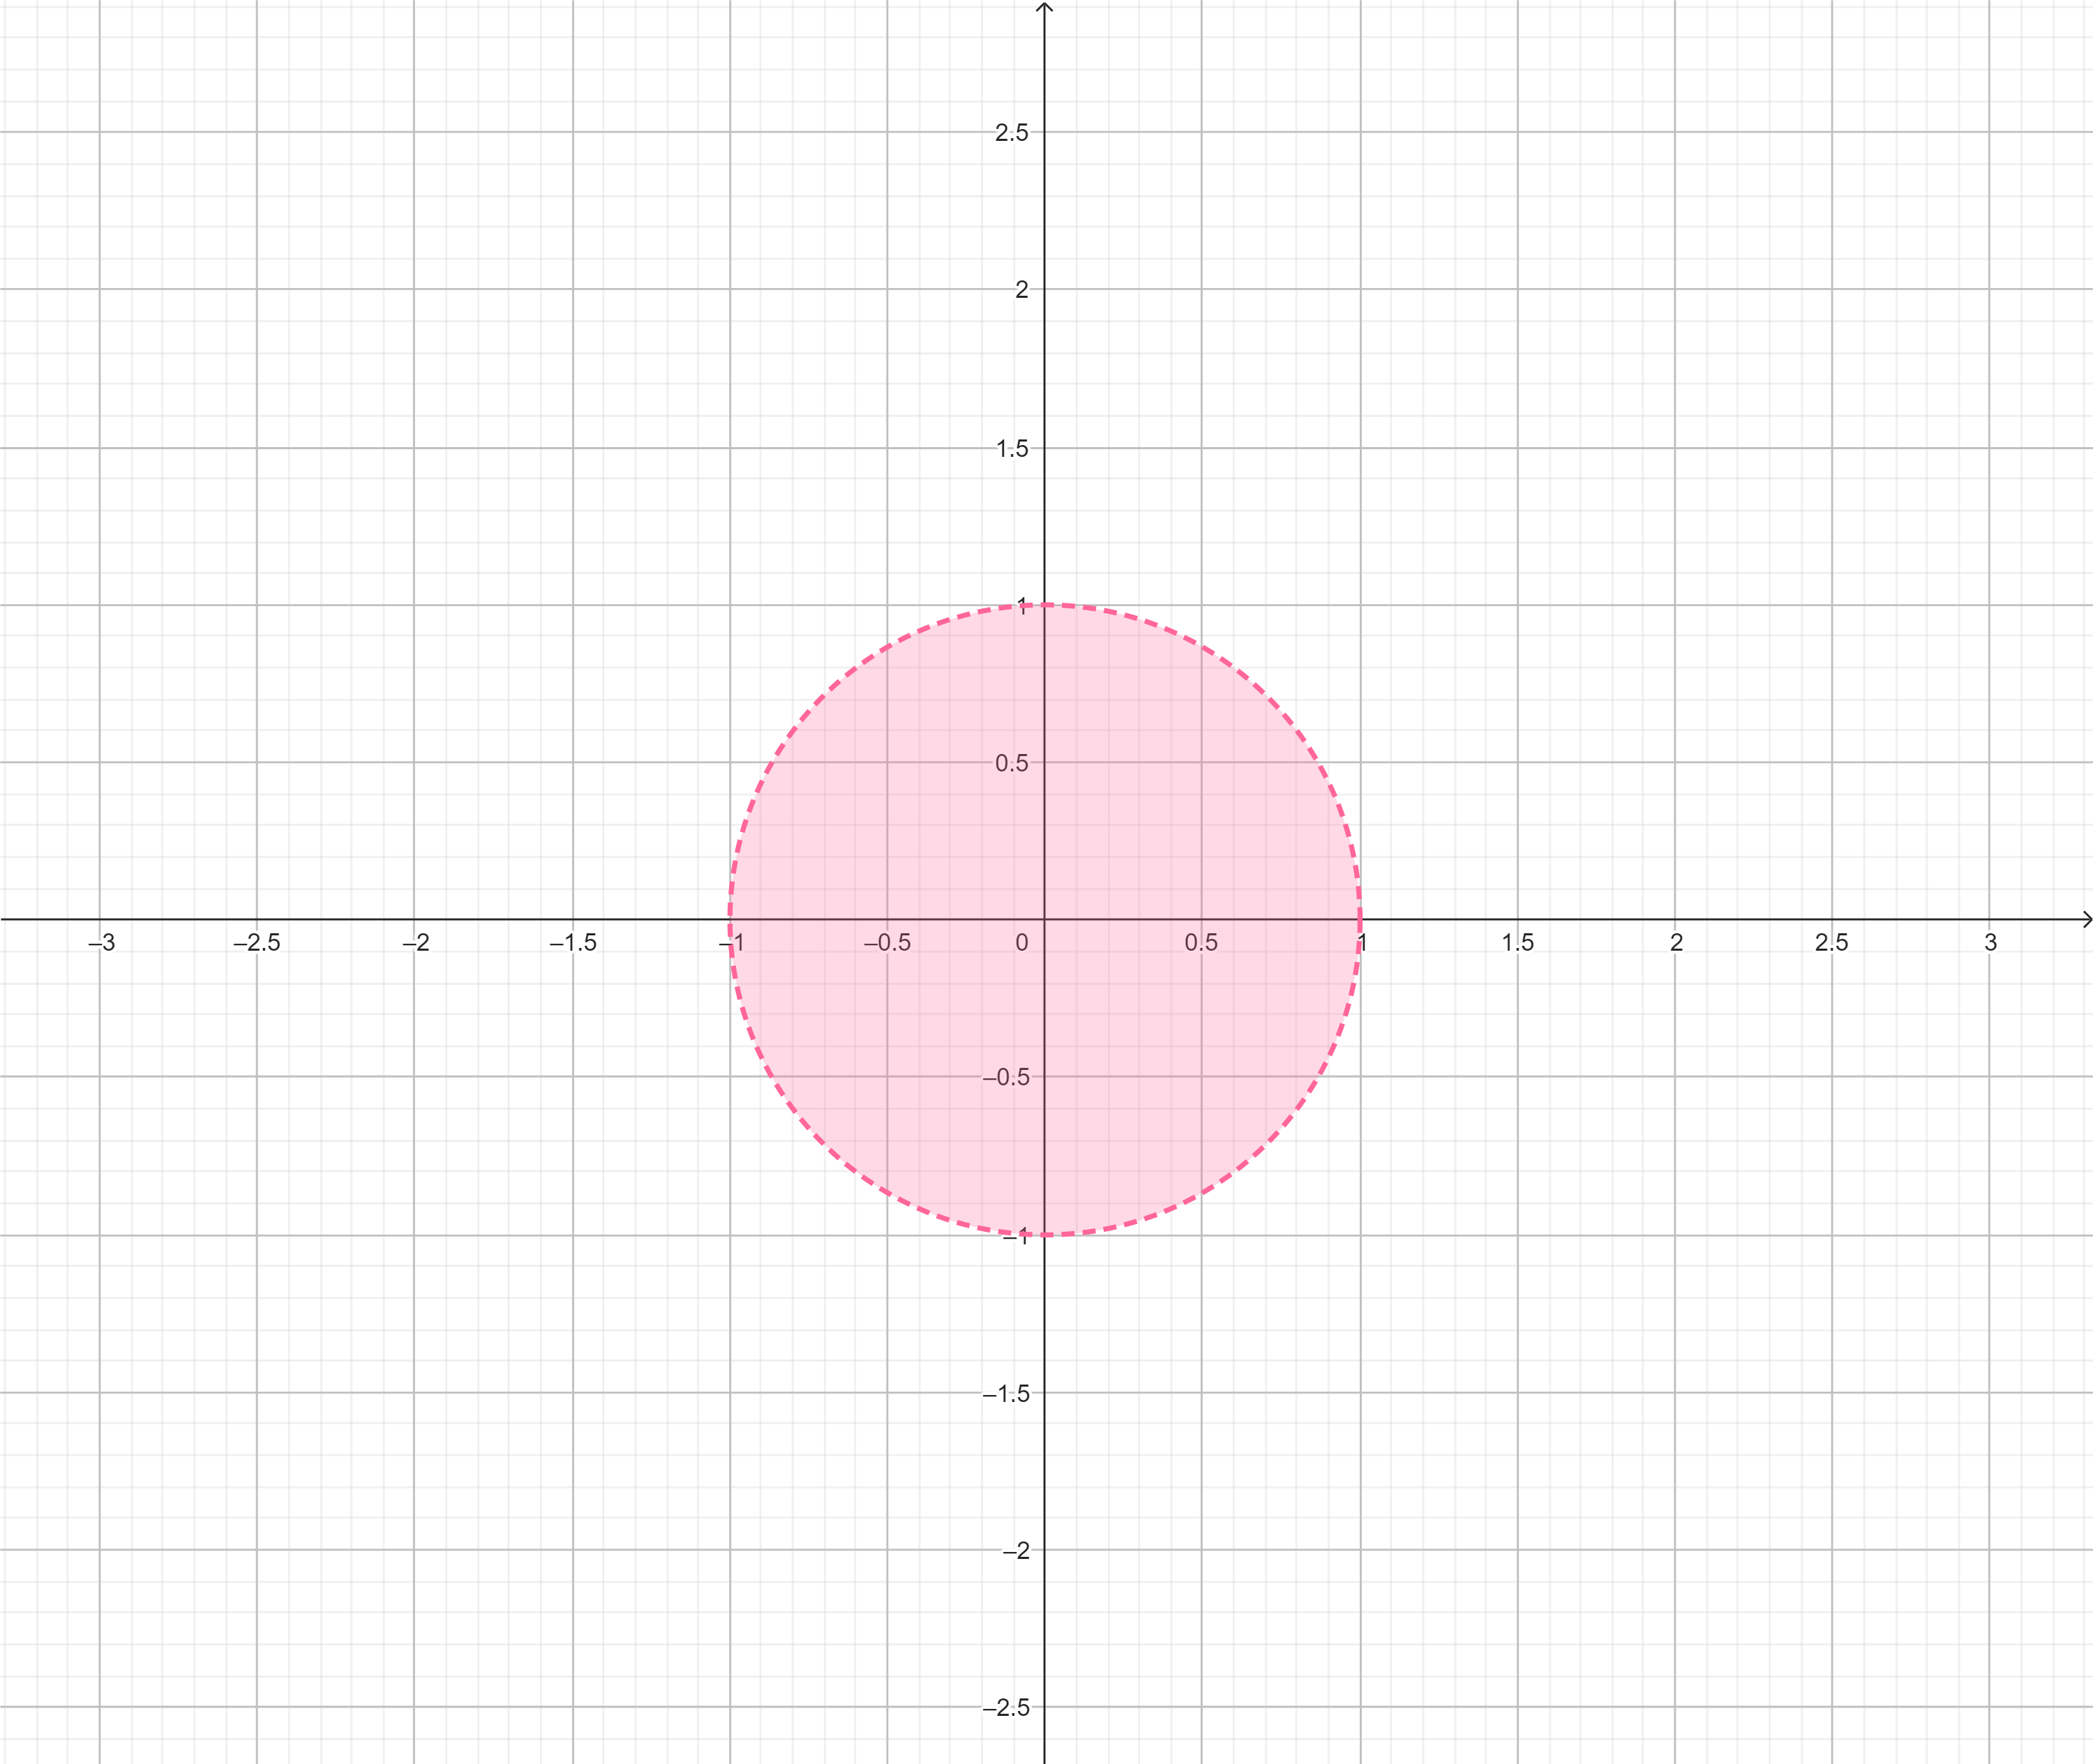
\includegraphics[scale=0.20] {graph1}
    	\caption{\label{fig:1} Open ball $B((0,0), 1) $ in $\alpha$ metric }
    \end{figure}
    
    
    \begin{figure}
    	\centering
    	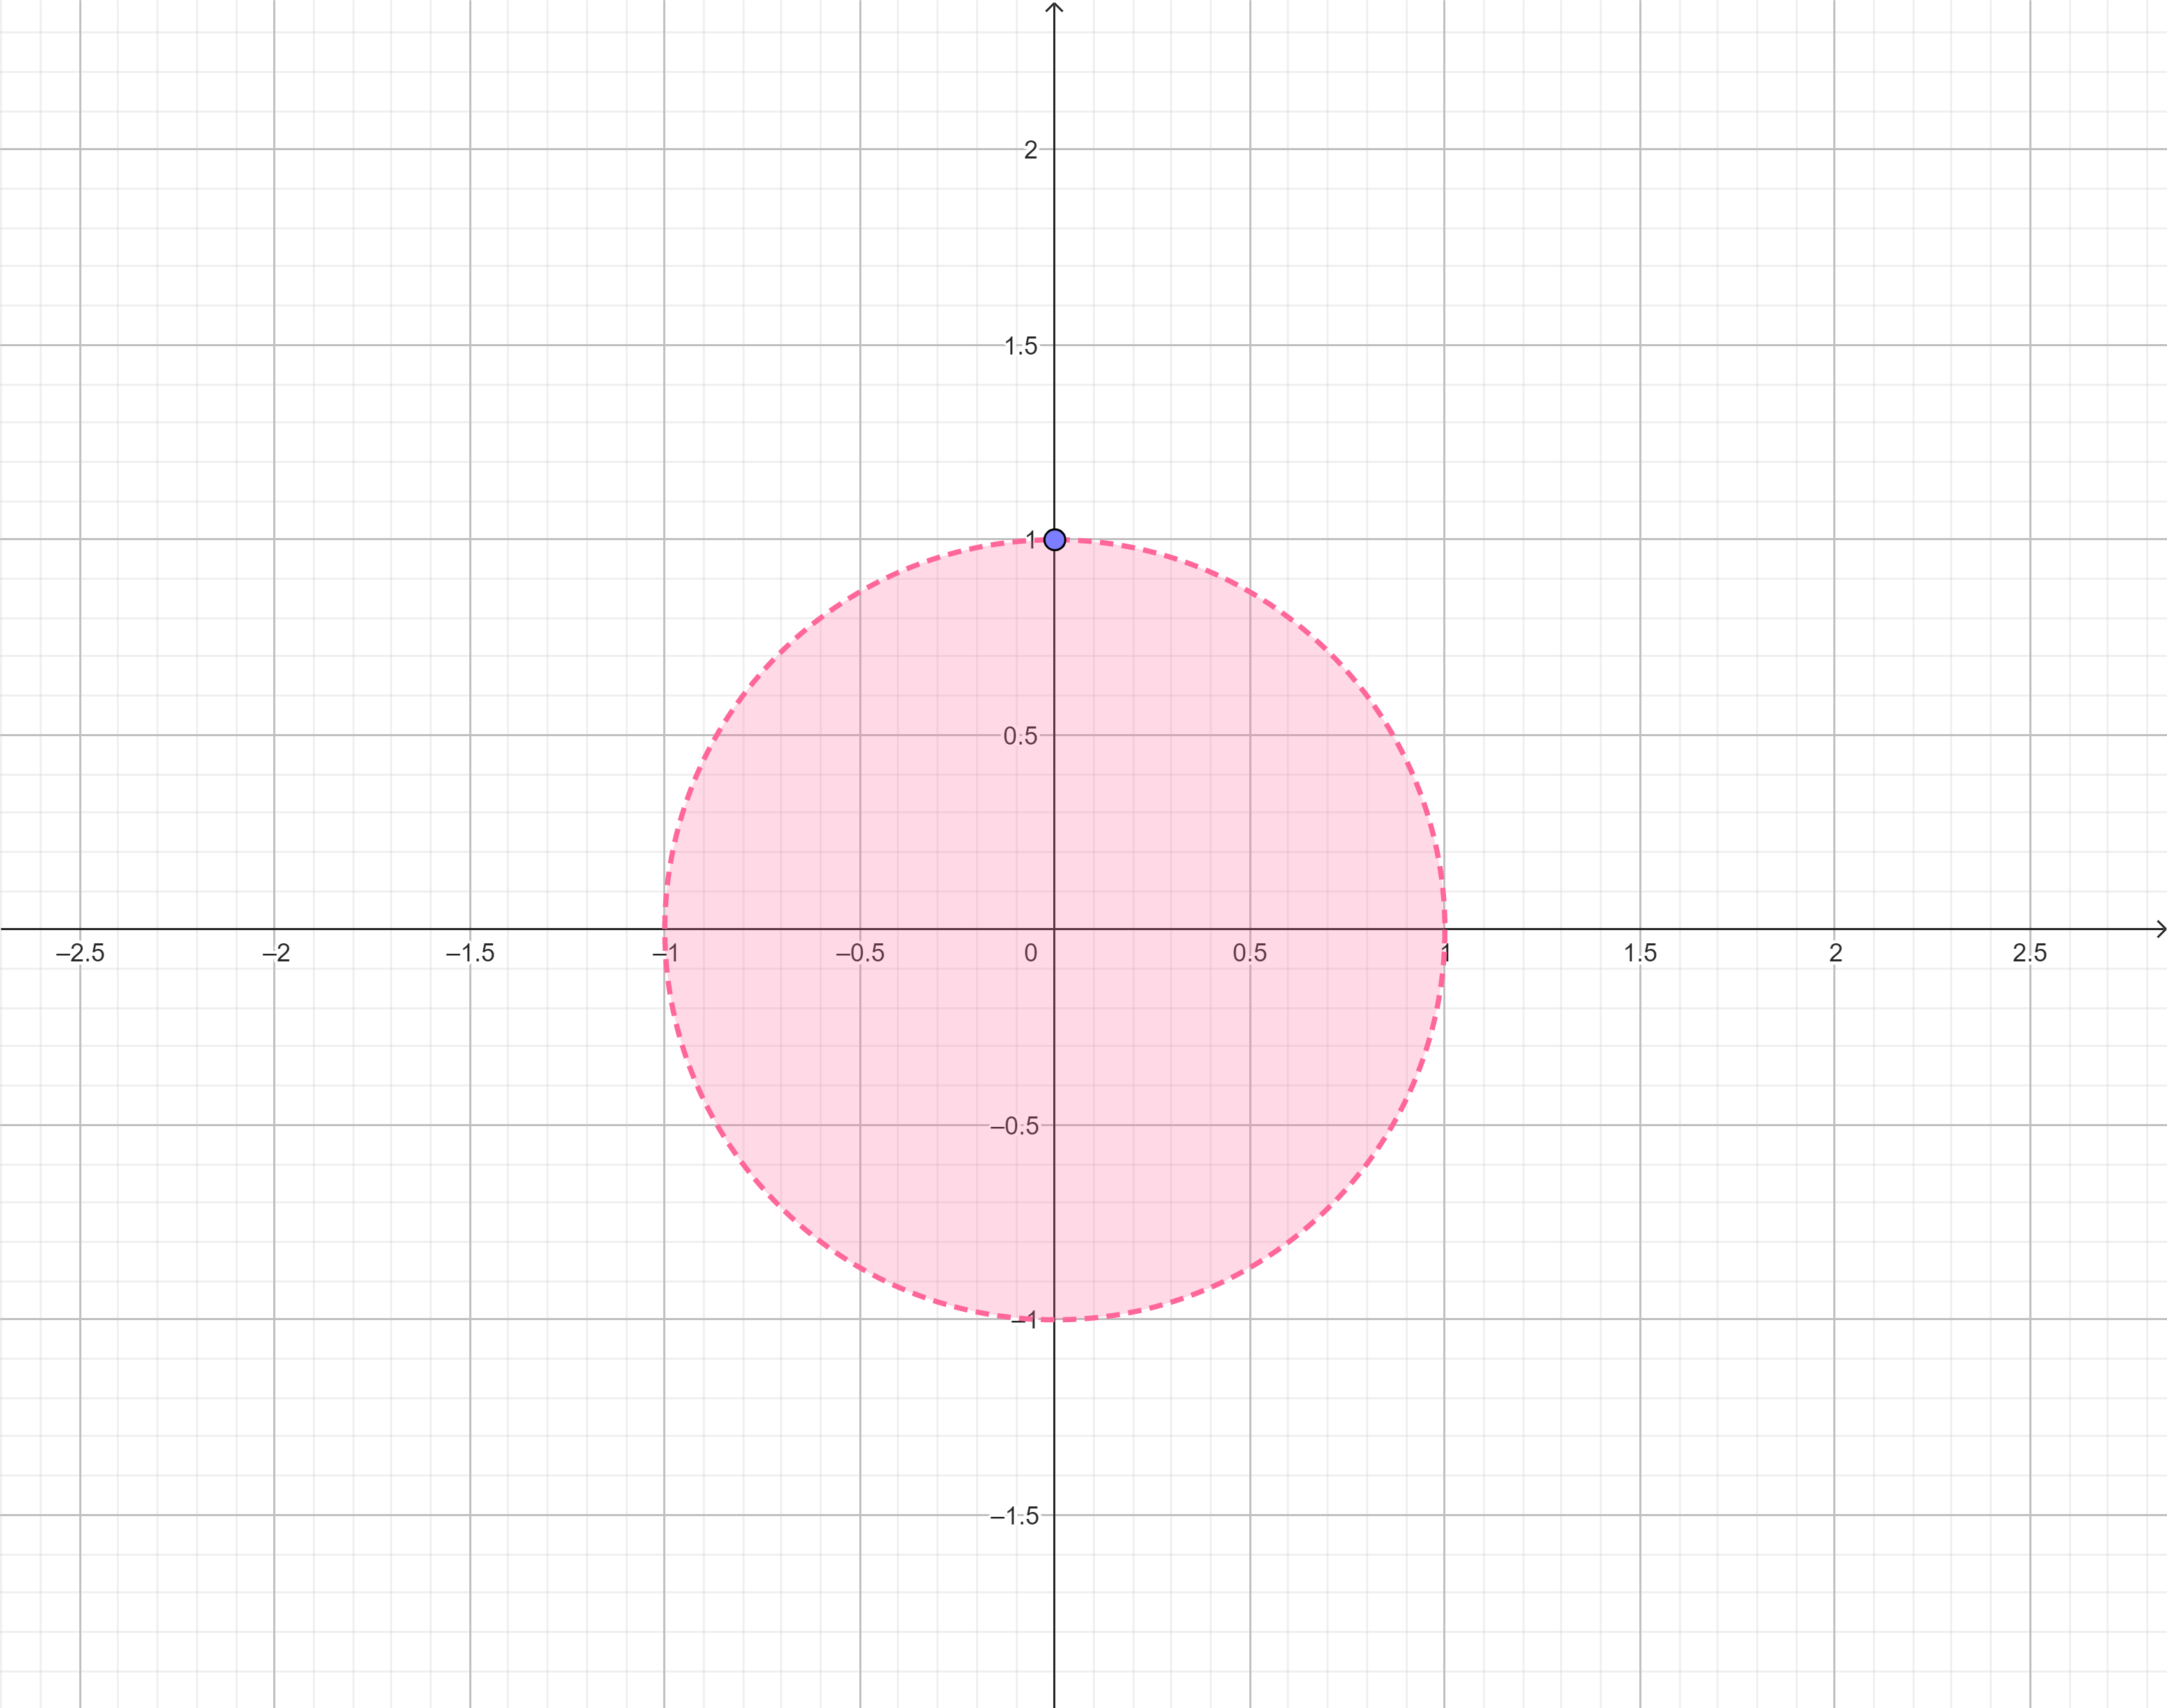
\includegraphics[scale=0.20] {graph2}
    	\caption{\label{fig:2} Open ball $B((0,1), 2) $ in $\alpha$ metric }
    \end{figure}

 \begin{figure}
	\centering
	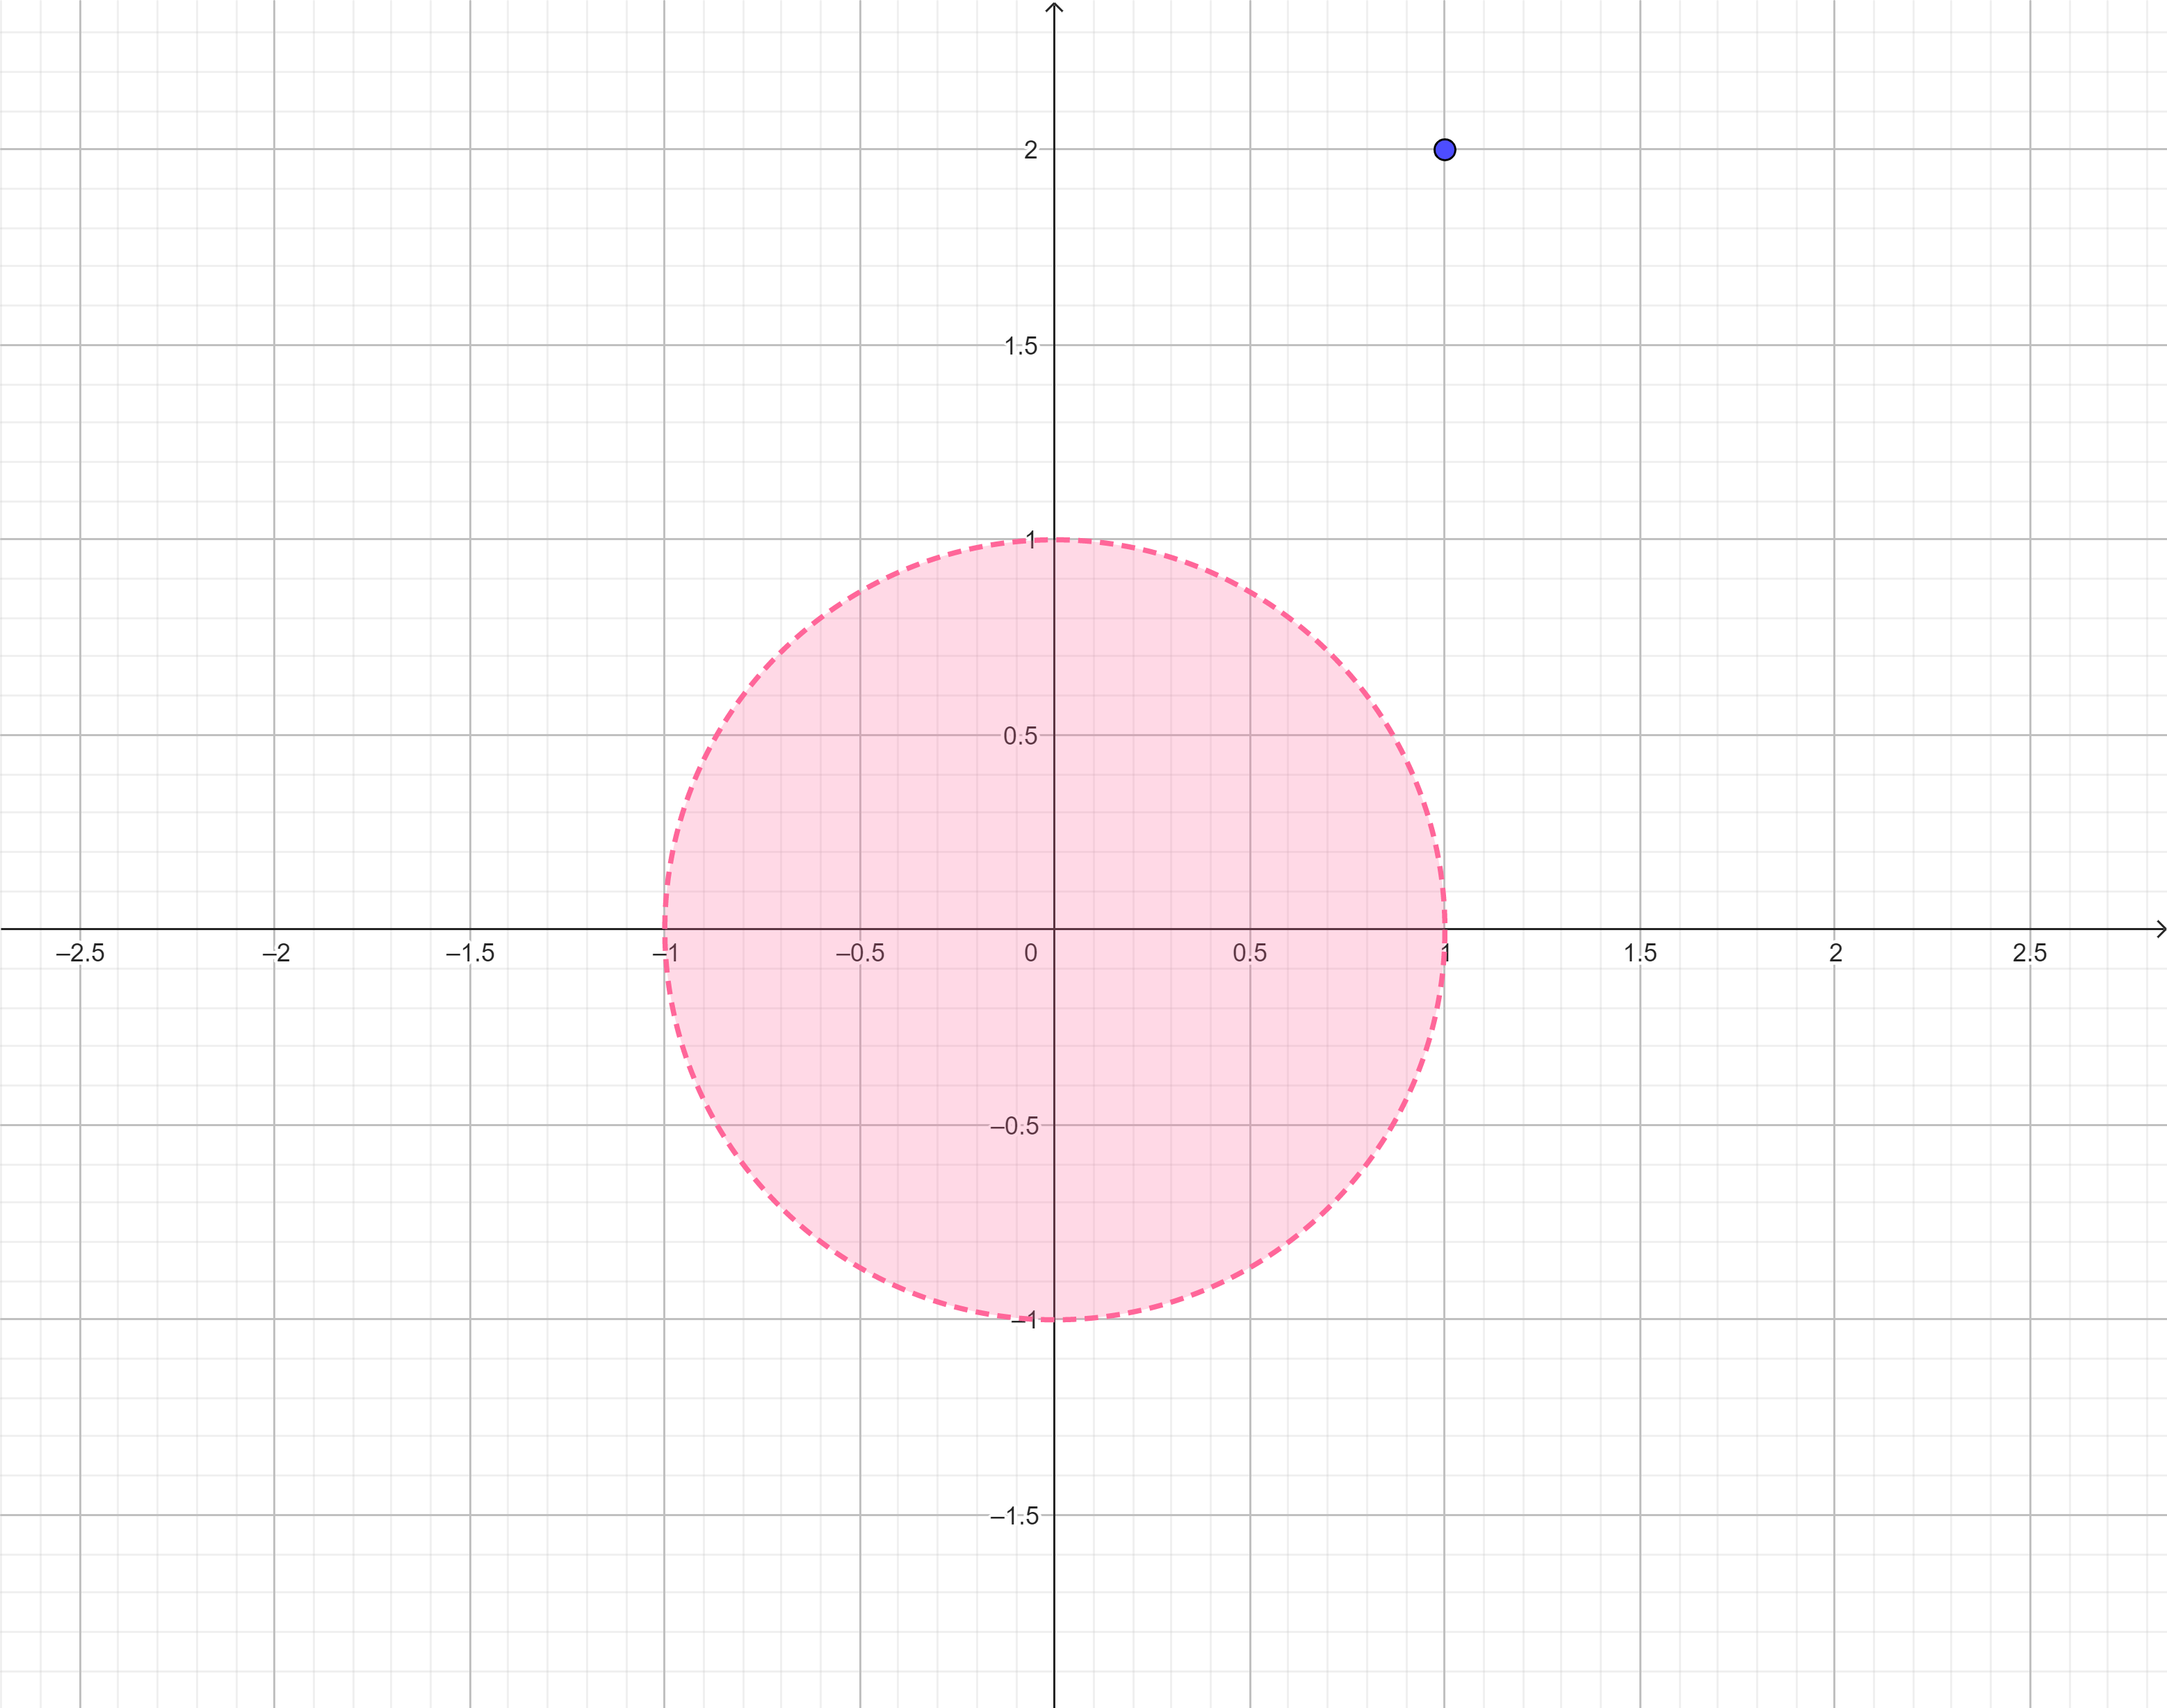
\includegraphics[scale=0.20] {graph3}
	\caption{\label{fig:2} Open ball $B((1,2), 1+\sqrt{5}) $ in $\alpha$ metric }
\end{figure}

	 


    \begin{align*} B((0,0), 1) &= \{(x_{1}, x_{2}) \in \mathbb{R}; \ \alpha((0,0),(x_{1}, x_{2}))<1\} \\
    &= \{(x_{1}, x_{2}) \in \mathbb{R}; \ x_{1} = 0 \land x_{2} = 0 \land 0 < 1 \} \cup \{(x_{1}, x_{2}) \in \mathbb{R}; \ x_{1} \neq 0 \lor x_{2} \neq 0 \land \sqrt{x_{1}^2 + x_{2}^2} < 1 \\
    &= \{(0,0) \} \cup \{(x_{1}, x_{2}) \in \mathbb{R}; \ x_{1} \neq 0 \lor x_{2} \neq 0 \land x_{1}^2 + x_{2}^2 < 1\} \\
     &= \{(x_{1}, x_{2}) \in \mathbb{R}; \ x_{1}^2 + x_{2}^2 < 1\} 
	\end{align*}
    
    \begin{align*} B((0,1), 2) &= \{(x_{1}, x_{2}) \in \mathbb{R}; \ \alpha((0,1),(x_{1}, x_{2}))<2\} \\
    	&= \{(x_{1}, x_{2}) \in \mathbb{R}; \ x_{1} = 0 \land x_{2} = 1 \land 0 < 2 \} \cup \{(x_{1}, x_{2}) \in \mathbb{R}; \ x_{1} \neq 0 \lor x_{2} \neq 1 \land \sqrt{0^2 + 1^2}  \\
    	&+ \sqrt{x_{1}^2 + x_{2}^2} < 2 \}\\
    	&= \{(0,1) \} \cup \{(x_{1}, x_{2}) \in \mathbb{R}; \ x_{1} \neq 0 \lor x_{2} \neq 1 \land \sqrt{1} + \sqrt{x_{1}^2 + x_{2}^2} < 2\} \\
    	&= \{(0,1) \} \cup \{(x_{1}, x_{2}) \in \mathbb{R}; \ \sqrt{x_{1}^2 + x_{2}^2} < 1\} \\
    	&= \{(0,1) \} \cup \{(x_{1}, x_{2}) \in \mathbb{R}; \ x_{1}^2 + x_{2}^2 < 1\}	
    \end{align*}

	\begin{align*} B((1,2), 1+\sqrt{5}) &= \{(x_{1}, x_{2}) \in \mathbb{R}; \ \alpha((1,2),(x_{1}, x_{2}))<1+\sqrt{5}\} \\
		&= \{(x_{1}, x_{2}) \in \mathbb{R}; \ x_{1} = 1 \land x_{2} = 2 \land 0 < 1 + \sqrt{5} \} \cup \{(x_{1}, x_{2}) \in \mathbb{R}; \ x_{1} \neq 1 \lor x_{2} \neq 2   \\
		&\land \sqrt{1^2 + 2^2} + \sqrt{x_{1}^2 + x_{2}^2} < 1 + \sqrt{5} \}\\
		&= \{(1,2) \} \cup \{(x_{1}, x_{2}) \in \mathbb{R}; \ x_{1} \neq 1 \lor x_{2} \neq 2 \land \sqrt{5} + \sqrt{x_{1}^2 + x_{2}^2} < 1 + \sqrt{5}\} \\
		&= \{(1,2) \} \cup \{(x_{1}, x_{2}) \in \mathbb{R}; \ \sqrt{x_{1}^2 + x_{2}^2} < 1\} \\
		&= \{(1,2) \} \cup \{(x_{1}, x_{2}) \in \mathbb{R}; \ x_{1}^2 + x_{2}^2 < 1\}	
	\end{align*}

	\textbf{(c)} I drew the open balls $B((0,0), 1)$, $B((0,1), 2)$ and $B((2,2), \sqrt{2})$ in $\beta$ metric. The drawings can be seen on Figures 4,5 and 6. The calculations I made were: 
	
	\begin{figure}
		\centering
		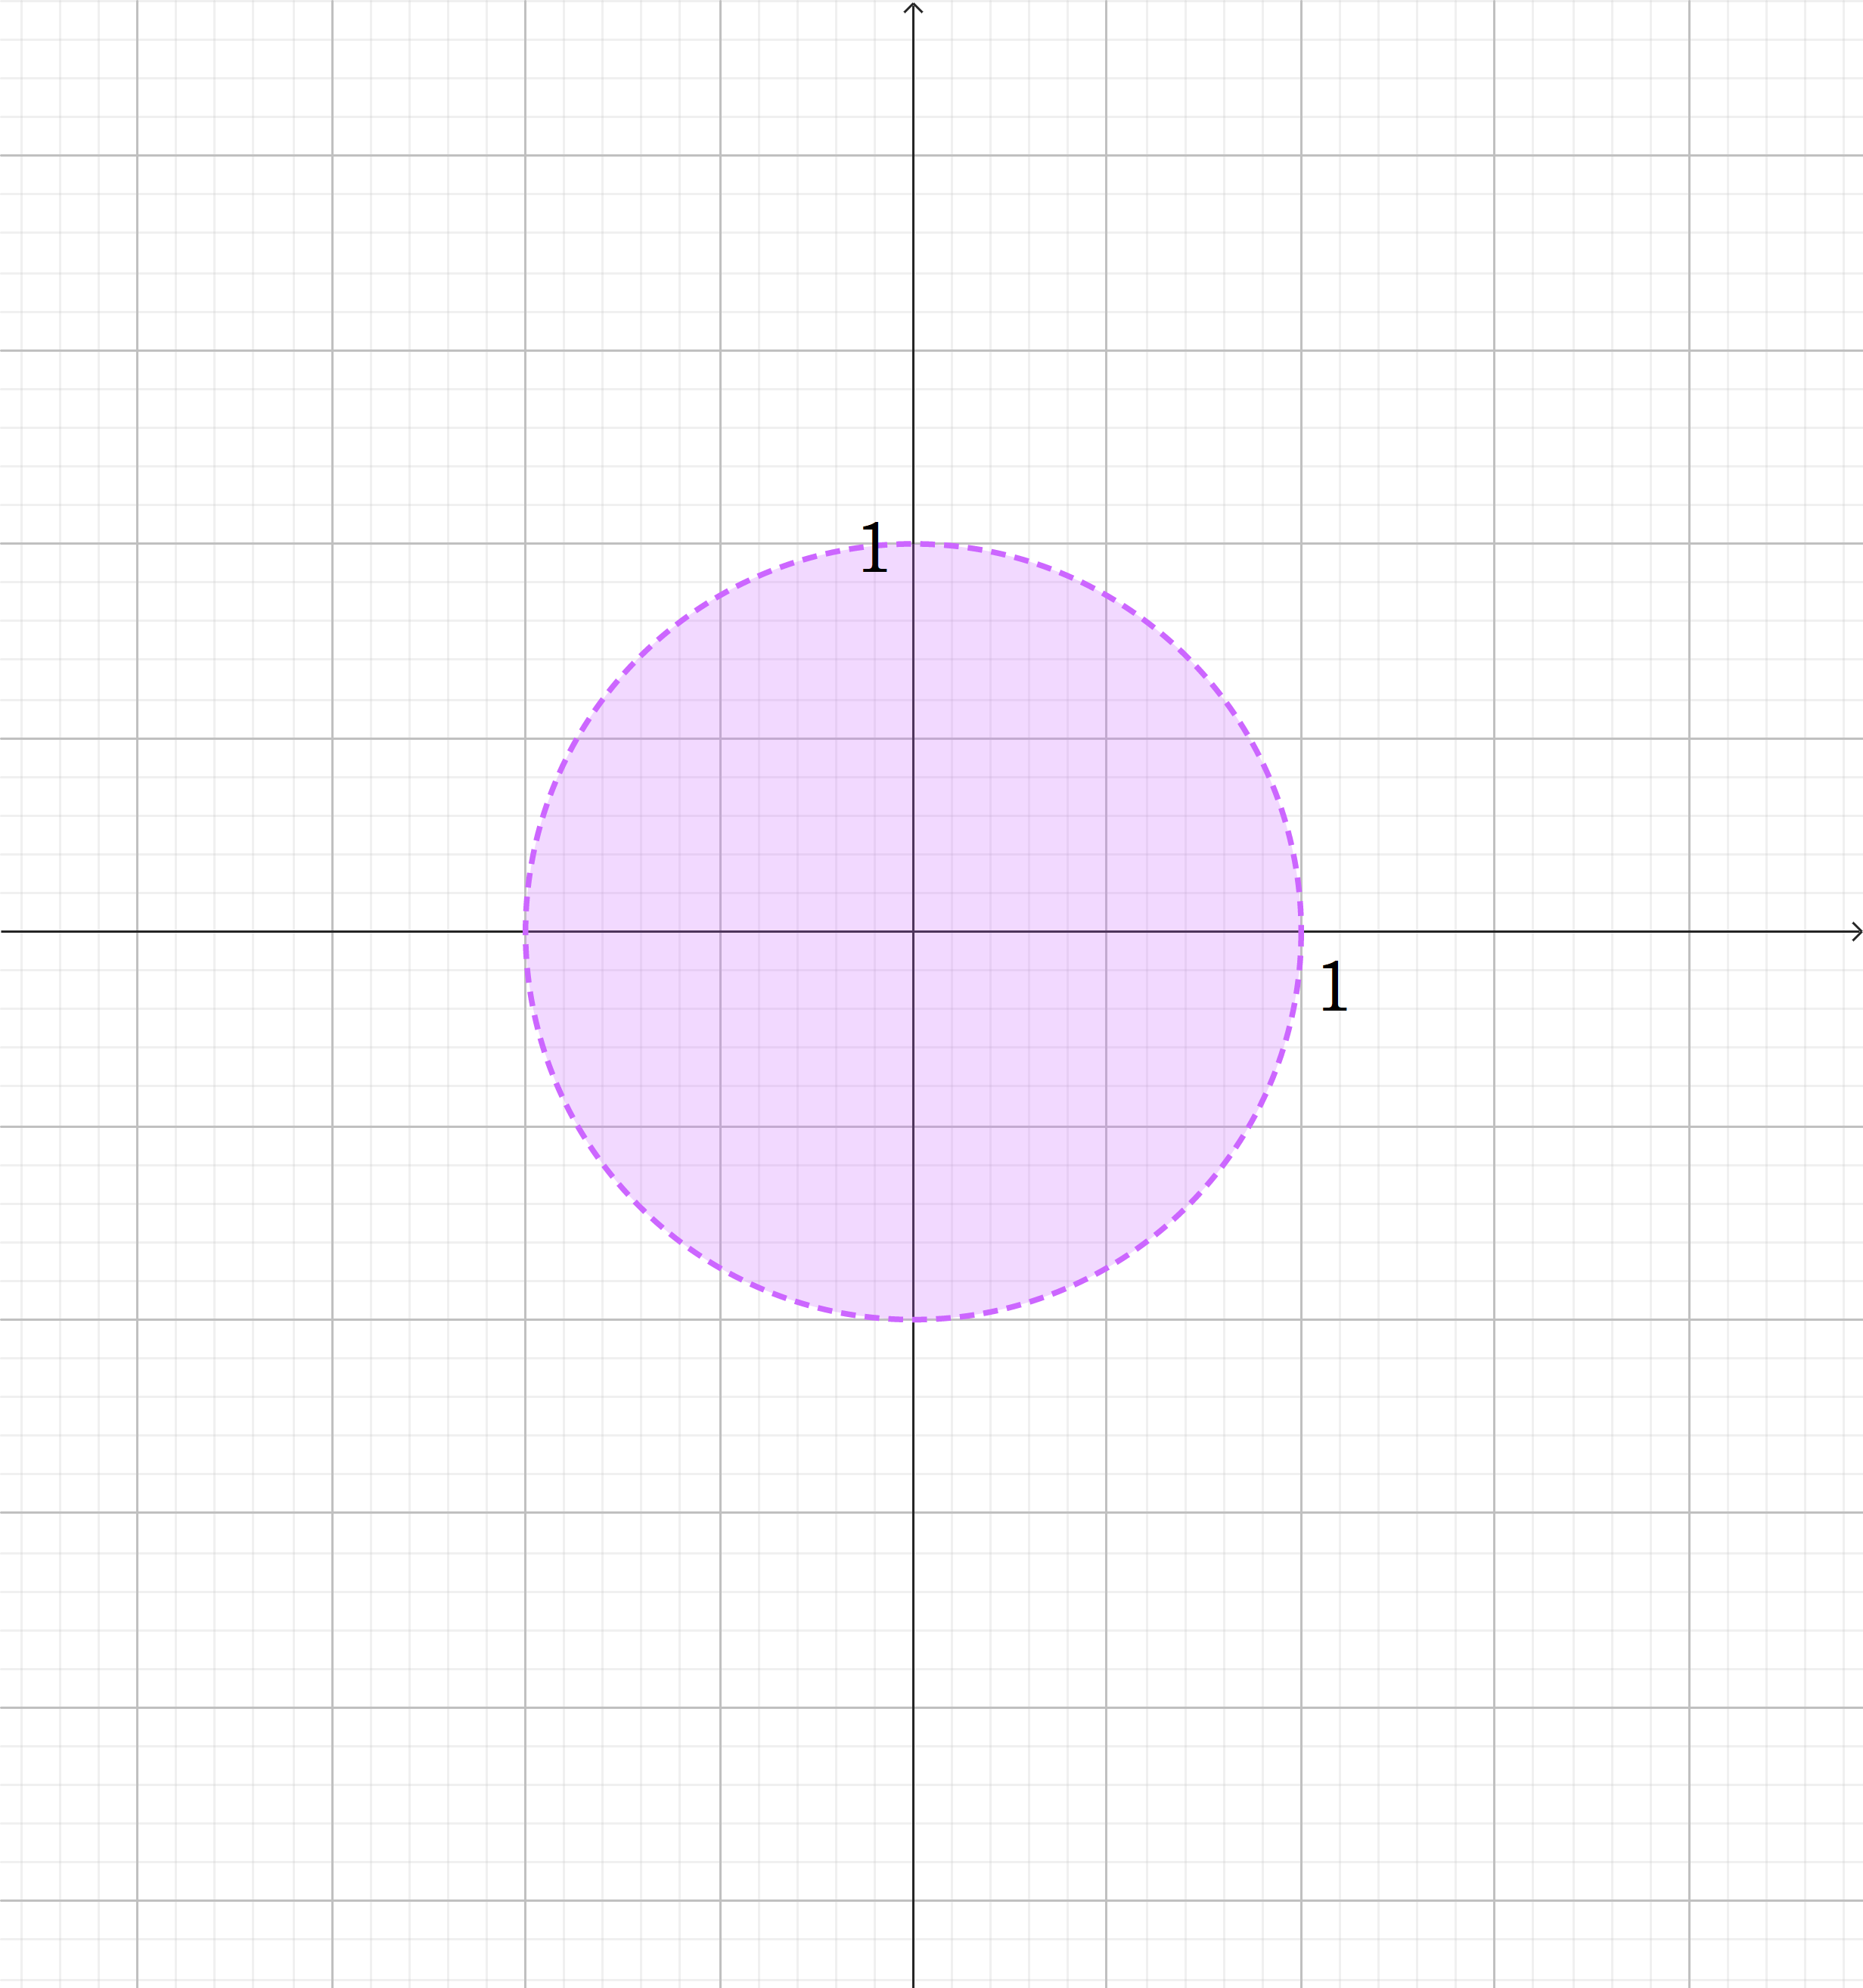
\includegraphics[scale=0.20] {graph4}
		\caption{\label{fig:4} Open ball $B((0,0), 1) $ in $\beta$ metric }
	\end{figure}
	
	
	\begin{figure}
		\centering
		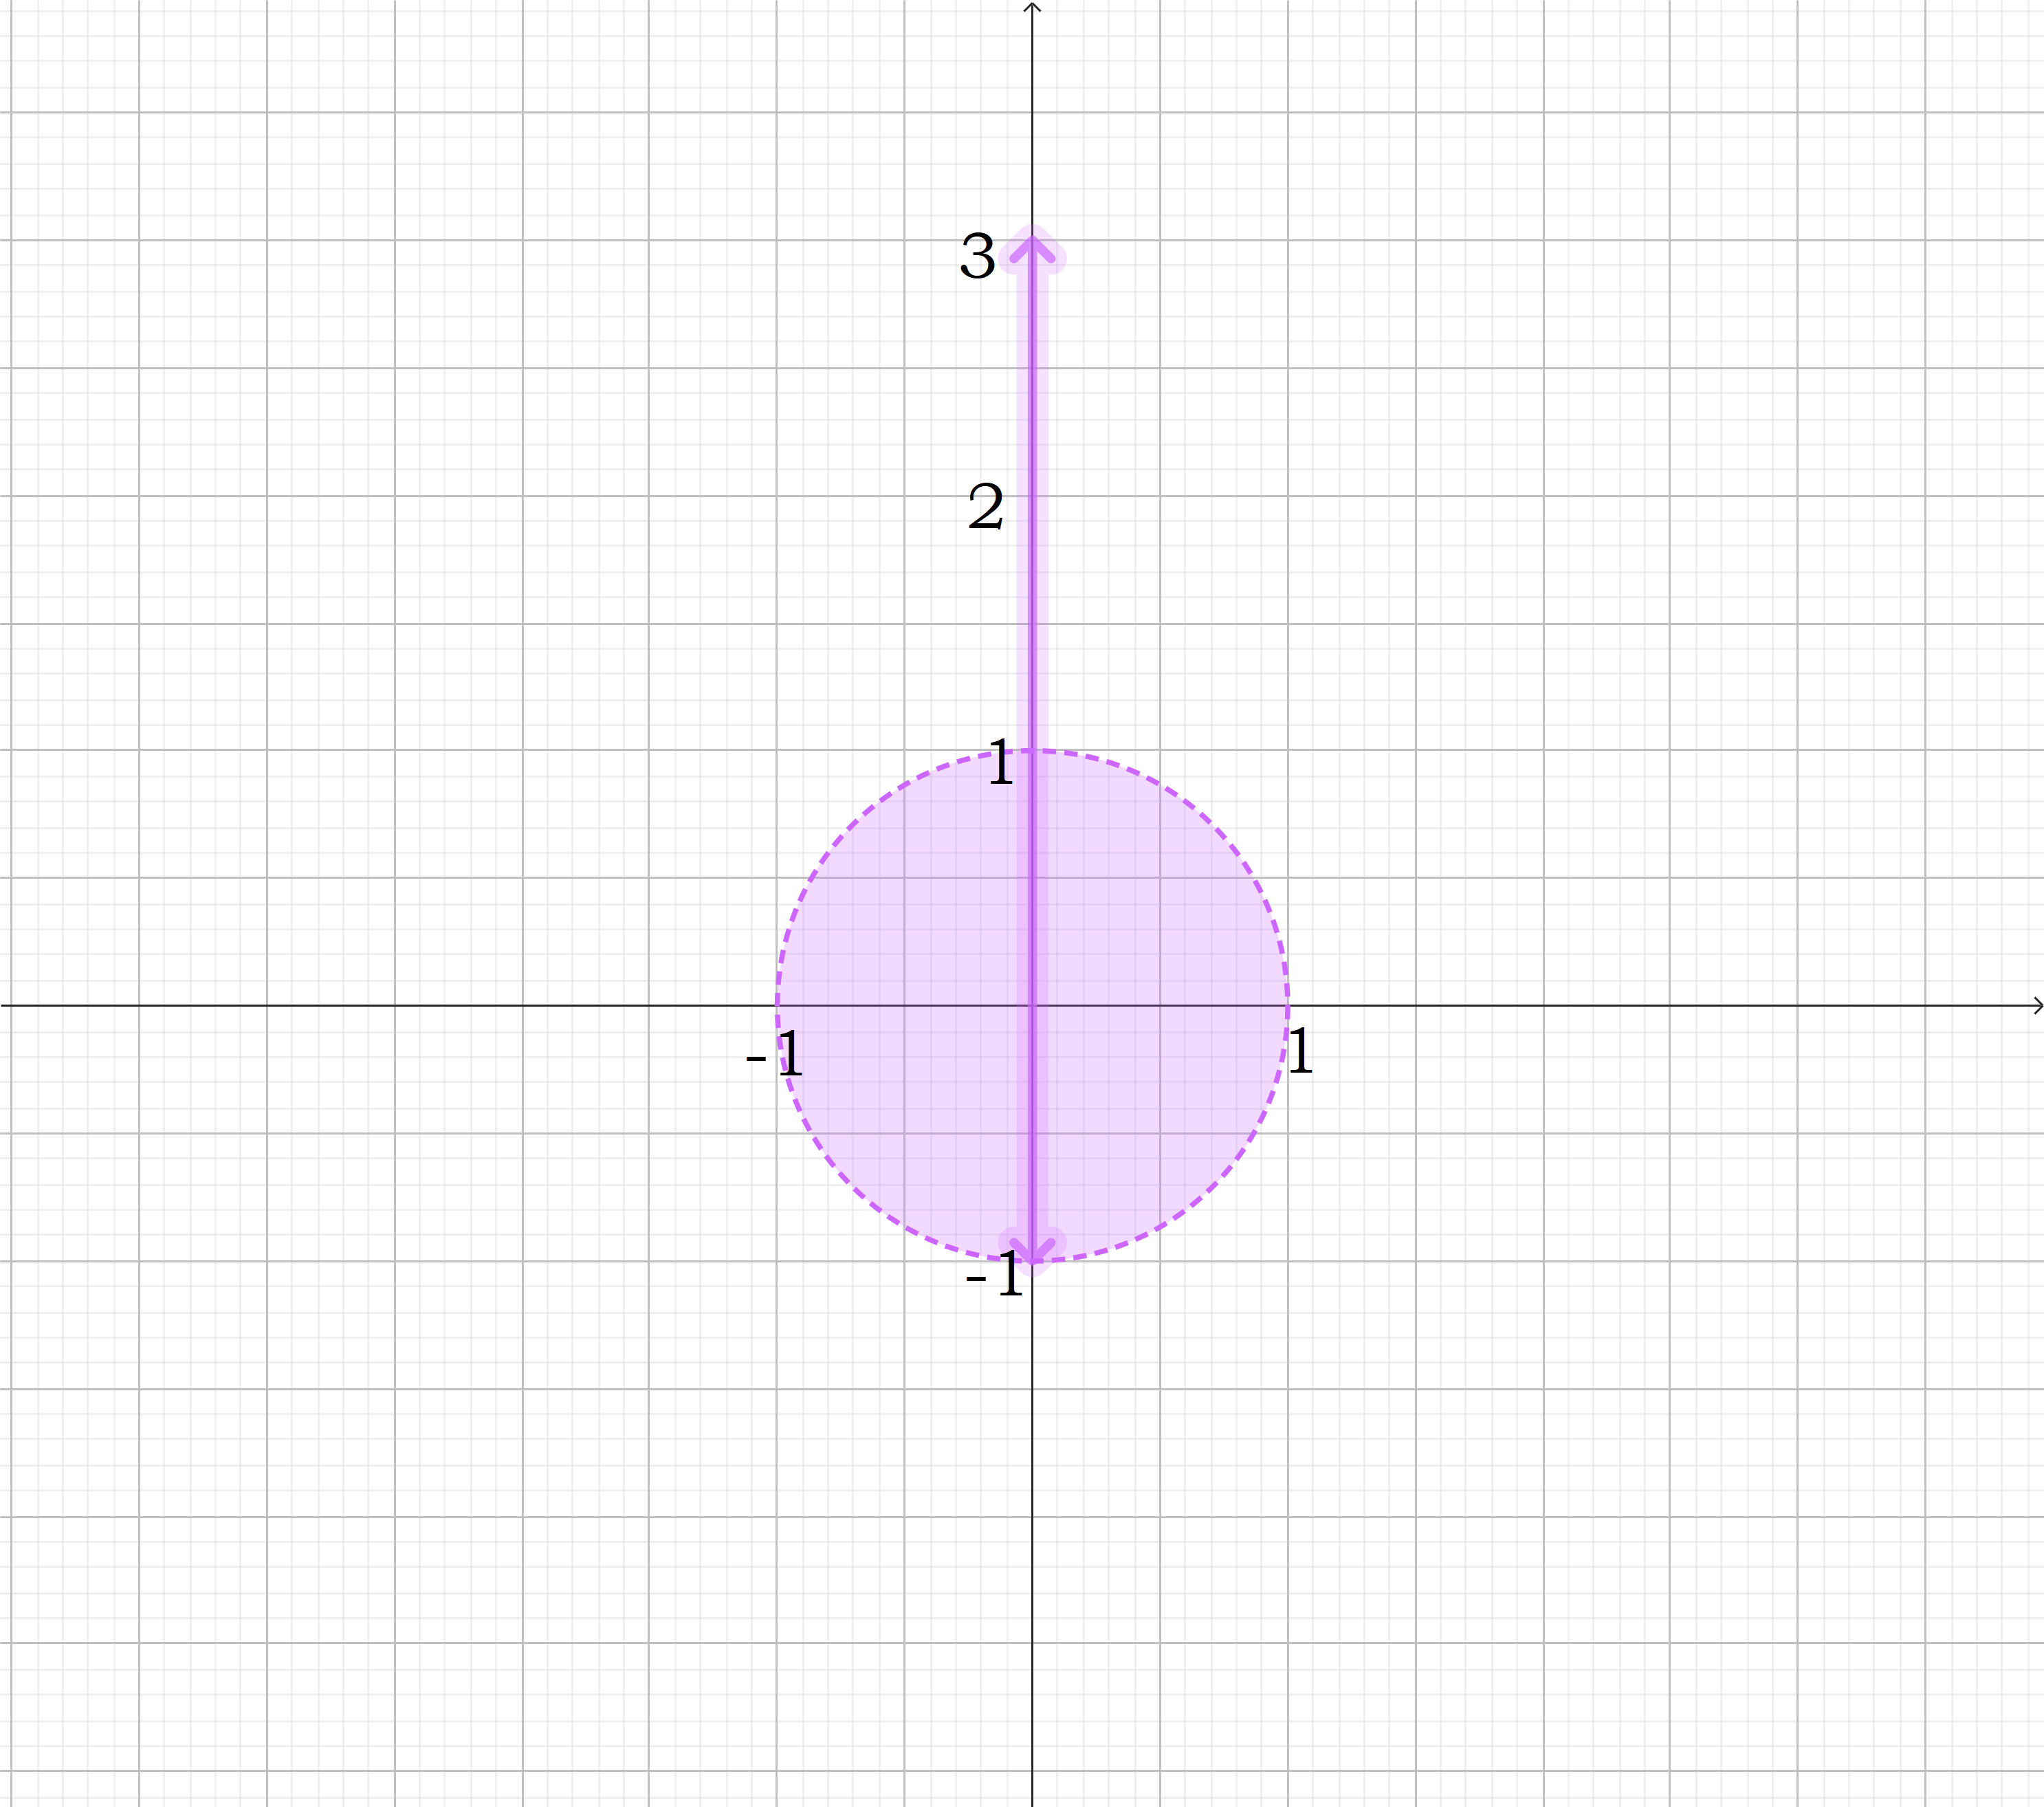
\includegraphics[scale=0.20] {graph5}
		\caption{\label{fig:5} Open ball $B((0,1), 2) $ in $\beta$ metric }
	\end{figure}
	
	\begin{figure}
		\centering
		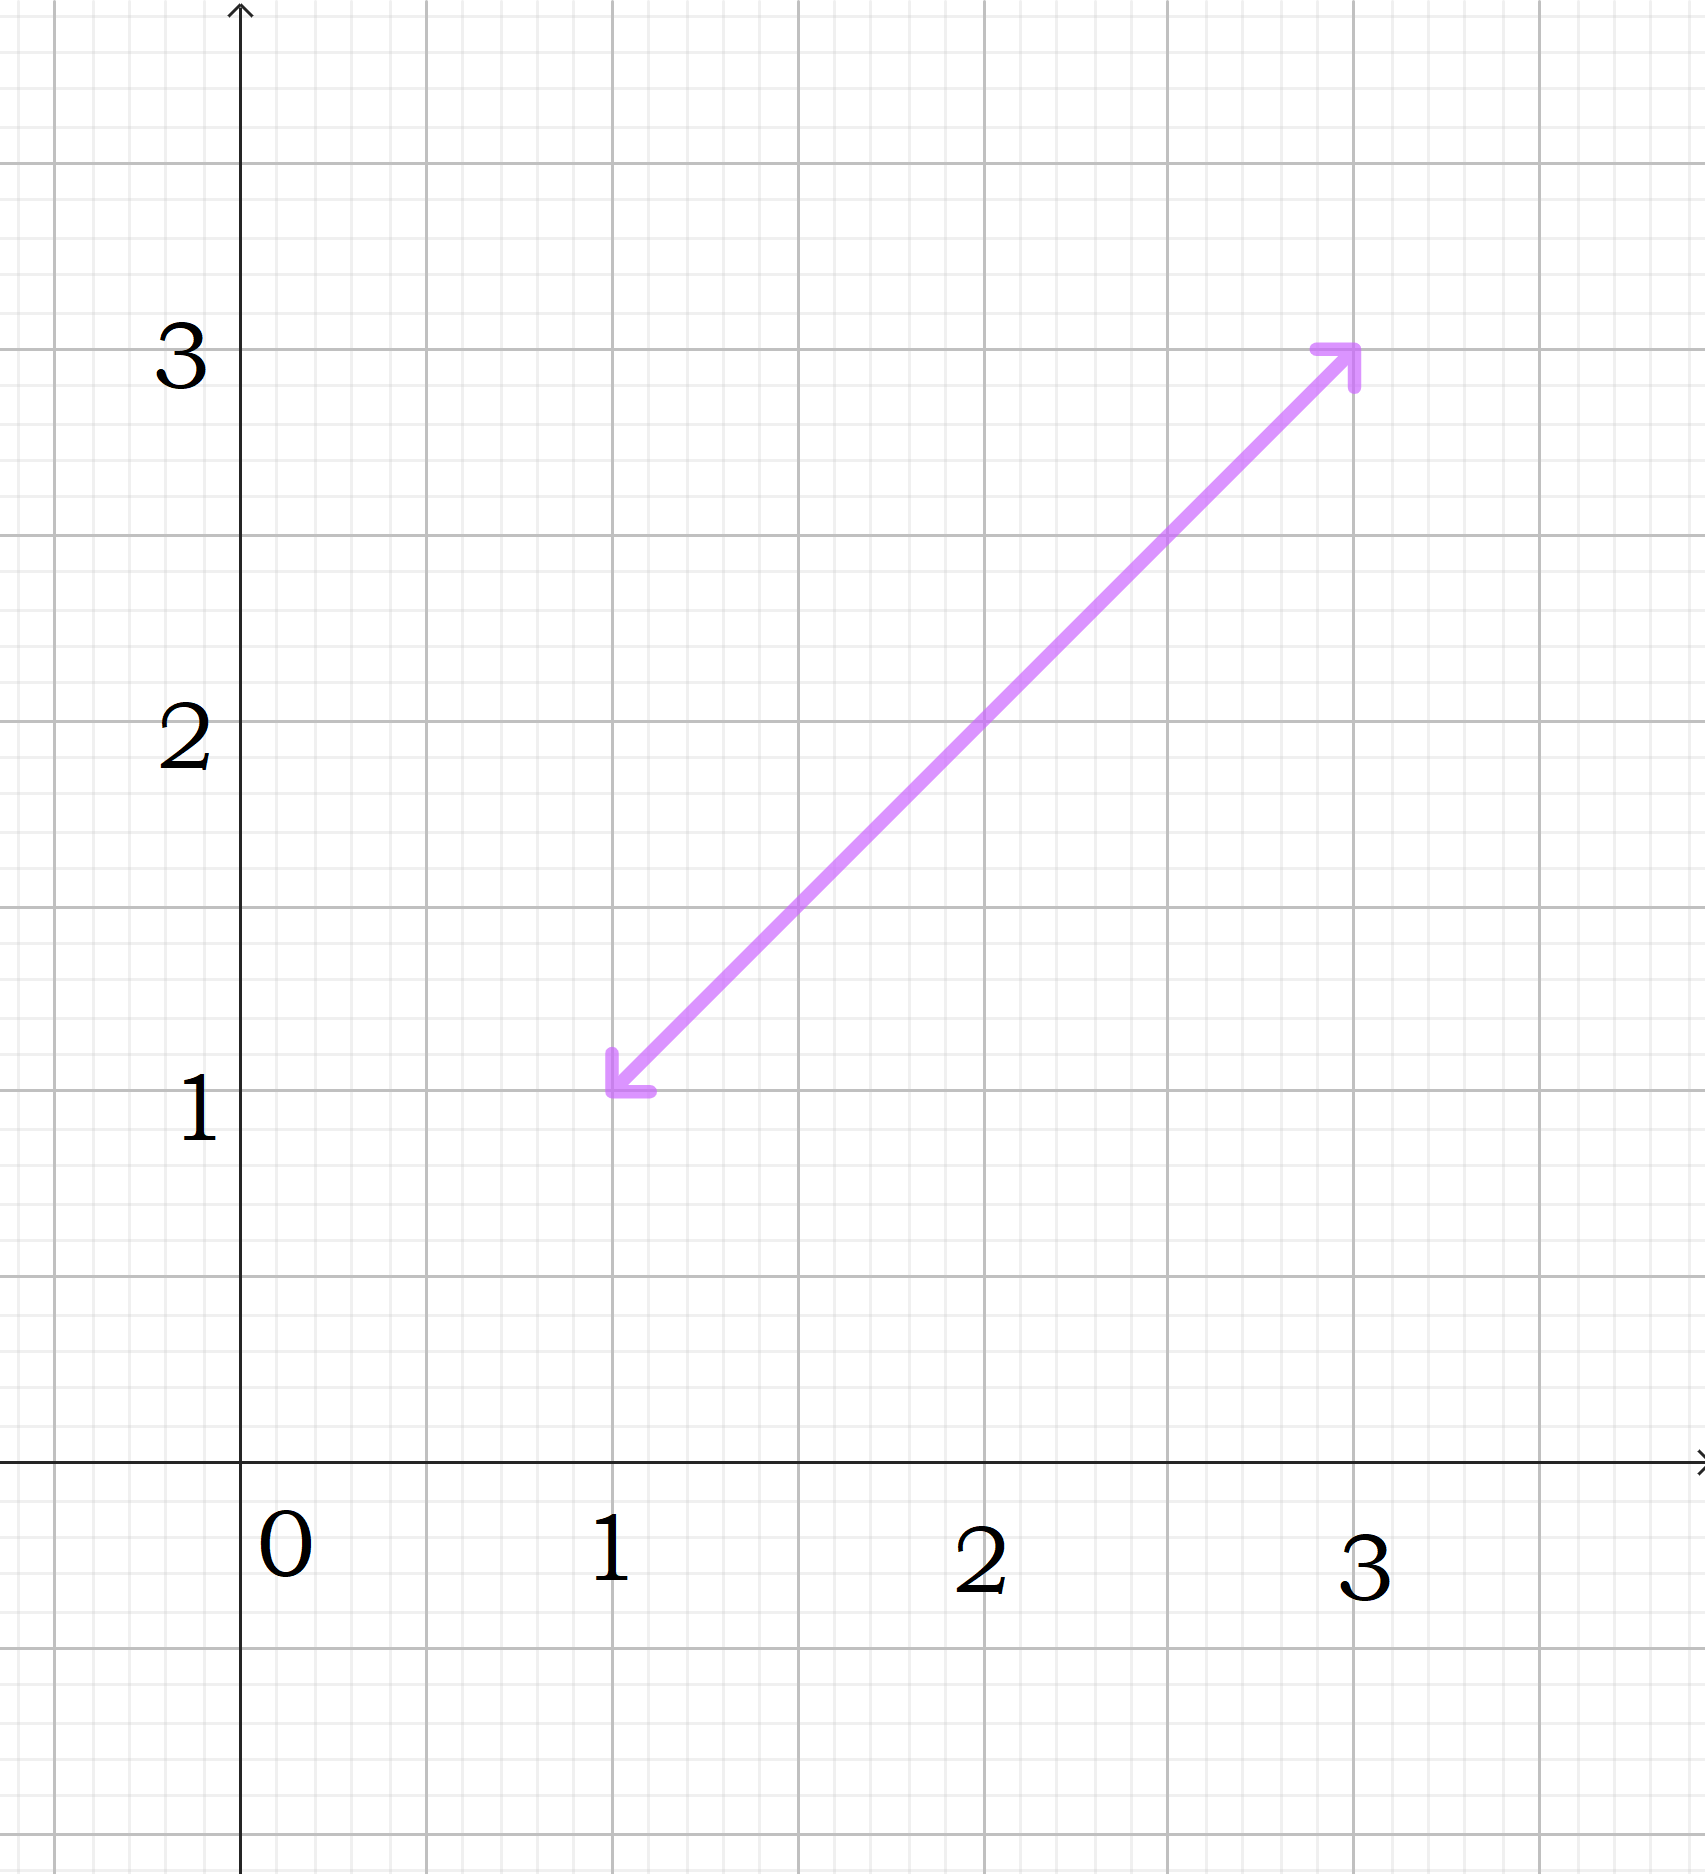
\includegraphics[scale=0.20] {graph6}
		\caption{\label{fig:6} Open ball $B((1,2), \sqrt{2}) $ in $\beta$ metric }
	\end{figure}
	
	\begin{align*} B((0,0), 1) &= \{(x_{1}, x_{2}) \in \mathbb{R}; \ \beta((0,0),(x_{1}, x_{2}))<1\} \\
		&= \{(x_{1}, x_{2}) \in \mathbb{R}; \ 0 \cdot x_{2} = 0 \cdot x_{1} \land  \sqrt{(0-x_{1})^2 + (0-x_{2})^2} < 1 \} \ \cup \\ 
		&\{(x_{1}, x_{2}) \in \mathbb{R}; \ 0 \cdot x_{2} \neq 0 \cdot x_{1} \land  \sqrt{0^2 + 0^2} + \sqrt{x_{1}^2 + x_{2}^2} < 1 \\
		&= \{(x_{1}, x_{2}) \in \mathbb{R}; \  \sqrt{(-x_{1})^2 + (-x_{2})^2} < 1 \} \cup \emptyset \\
		&= \{(x_{1}, x_{2}) \in \mathbb{R}; \ x_{1}^2 + x_{2}^2 < 1\} 
	\end{align*}

	\begin{align*} B((0,1), 2) &= \{(x_{1}, x_{2}) \in \mathbb{R}; \ \beta((0,1),(x_{1}, x_{2}))<2\} \\
		&= \{(x_{1}, x_{2}) \in \mathbb{R}; \ 0 \cdot x_{2} = 1 \cdot x_{1} \land  \sqrt{(0-x_{1})^2 + (1-x_{2})^2} < 2 \} \ \cup \\ 
		&\{(x_{1}, x_{2}) \in \mathbb{R}; \ 0 \cdot x_{2} \neq 1 \cdot x_{1} \land  \sqrt{0^2 + 1^2} + \sqrt{x_{1}^2 + x_{2}^2} < 2 \} \\
		&=\{(x_{1}, x_{2}) \in \mathbb{R}; \ x_{1} = 0 \land  \sqrt{(1-x_{2})^2} < 2 \} \ \cup 
		\{(x_{1}, x_{2}) \in \mathbb{R}; \ x_{1} \neq 0 \land  \sqrt{1} + \sqrt{x_{1}^2 + x_{2}^2} < 2 \} \\ 
		&=\{(x_{1}, x_{2}) \in \mathbb{R}; \ x_{1} = 0 \land  |1-x_{2}| < 2 \} \ \cup 
		\{(x_{1}, x_{2}) \in \mathbb{R}; \ x_{1} \neq 0 \land \sqrt{x_{1}^2 + x_{2}^2} < 1 \} \\ 
		&=\{(0, x_{2}) \in \mathbb{R}; |1-x_{2}| < 2 \} \ \cup 
		\{(x_{1}, x_{2}) \in \mathbb{R}; \ x_{1} \neq 0 \land x_{1}^2 + x_{2}^2 < 1 \}
	\end{align*}

	\begin{align*} B((2,2), \sqrt{2}) &= \{(x_{1}, x_{2}) \in \mathbb{R}; \ \beta((2,2),(x_{1}, x_{2}))<\sqrt{2}\} \\
		&= \{(x_{1}, x_{2}) \in \mathbb{R}; \ 2 \cdot x_{2} = 2 \cdot x_{1} \land  \sqrt{(2-x_{1})^2 + (2-x_{2})^2} < \sqrt{2} \} \ \cup \\ 
		&\{(x_{1}, x_{2}) \in \mathbb{R}; \ 2 \cdot x_{2} \neq 2 \cdot x_{1} \land  \sqrt{2^2 + 2^2} + \sqrt{x_{1}^2 + x_{2}^2} < \sqrt{2} \} \\
		&=\{(x_{1}, x_{2}) \in \mathbb{R}; \ \cdot x_{1} = x_{2} \land  \sqrt{2\cdot(2-x_{2})^2} < \sqrt{2} \} \\
		&\cup 
		\{(x_{1}, x_{2}) \in \mathbb{R}; \ x_{1} \neq x_{2} \land \sqrt{8} + \sqrt{x_{1}^2 + x_{2}^2} < \sqrt{2} \} \\ 
		&=\{(x_{1}, x_{1}) \in \mathbb{R}; \ |2-x_{1}| < 2 \} \ \cup \emptyset
	\end{align*}

	\textbf{(d)} I drew the open balls $B((0,0), 1)$, $B((0,1), 2)$ and $B((2,2), \sqrt{2})$ in $\gamma$ metric. The drawings can be seen on Figures 7,8 and 9. The calculations I made were: 
	
		\begin{figure}
		\centering
		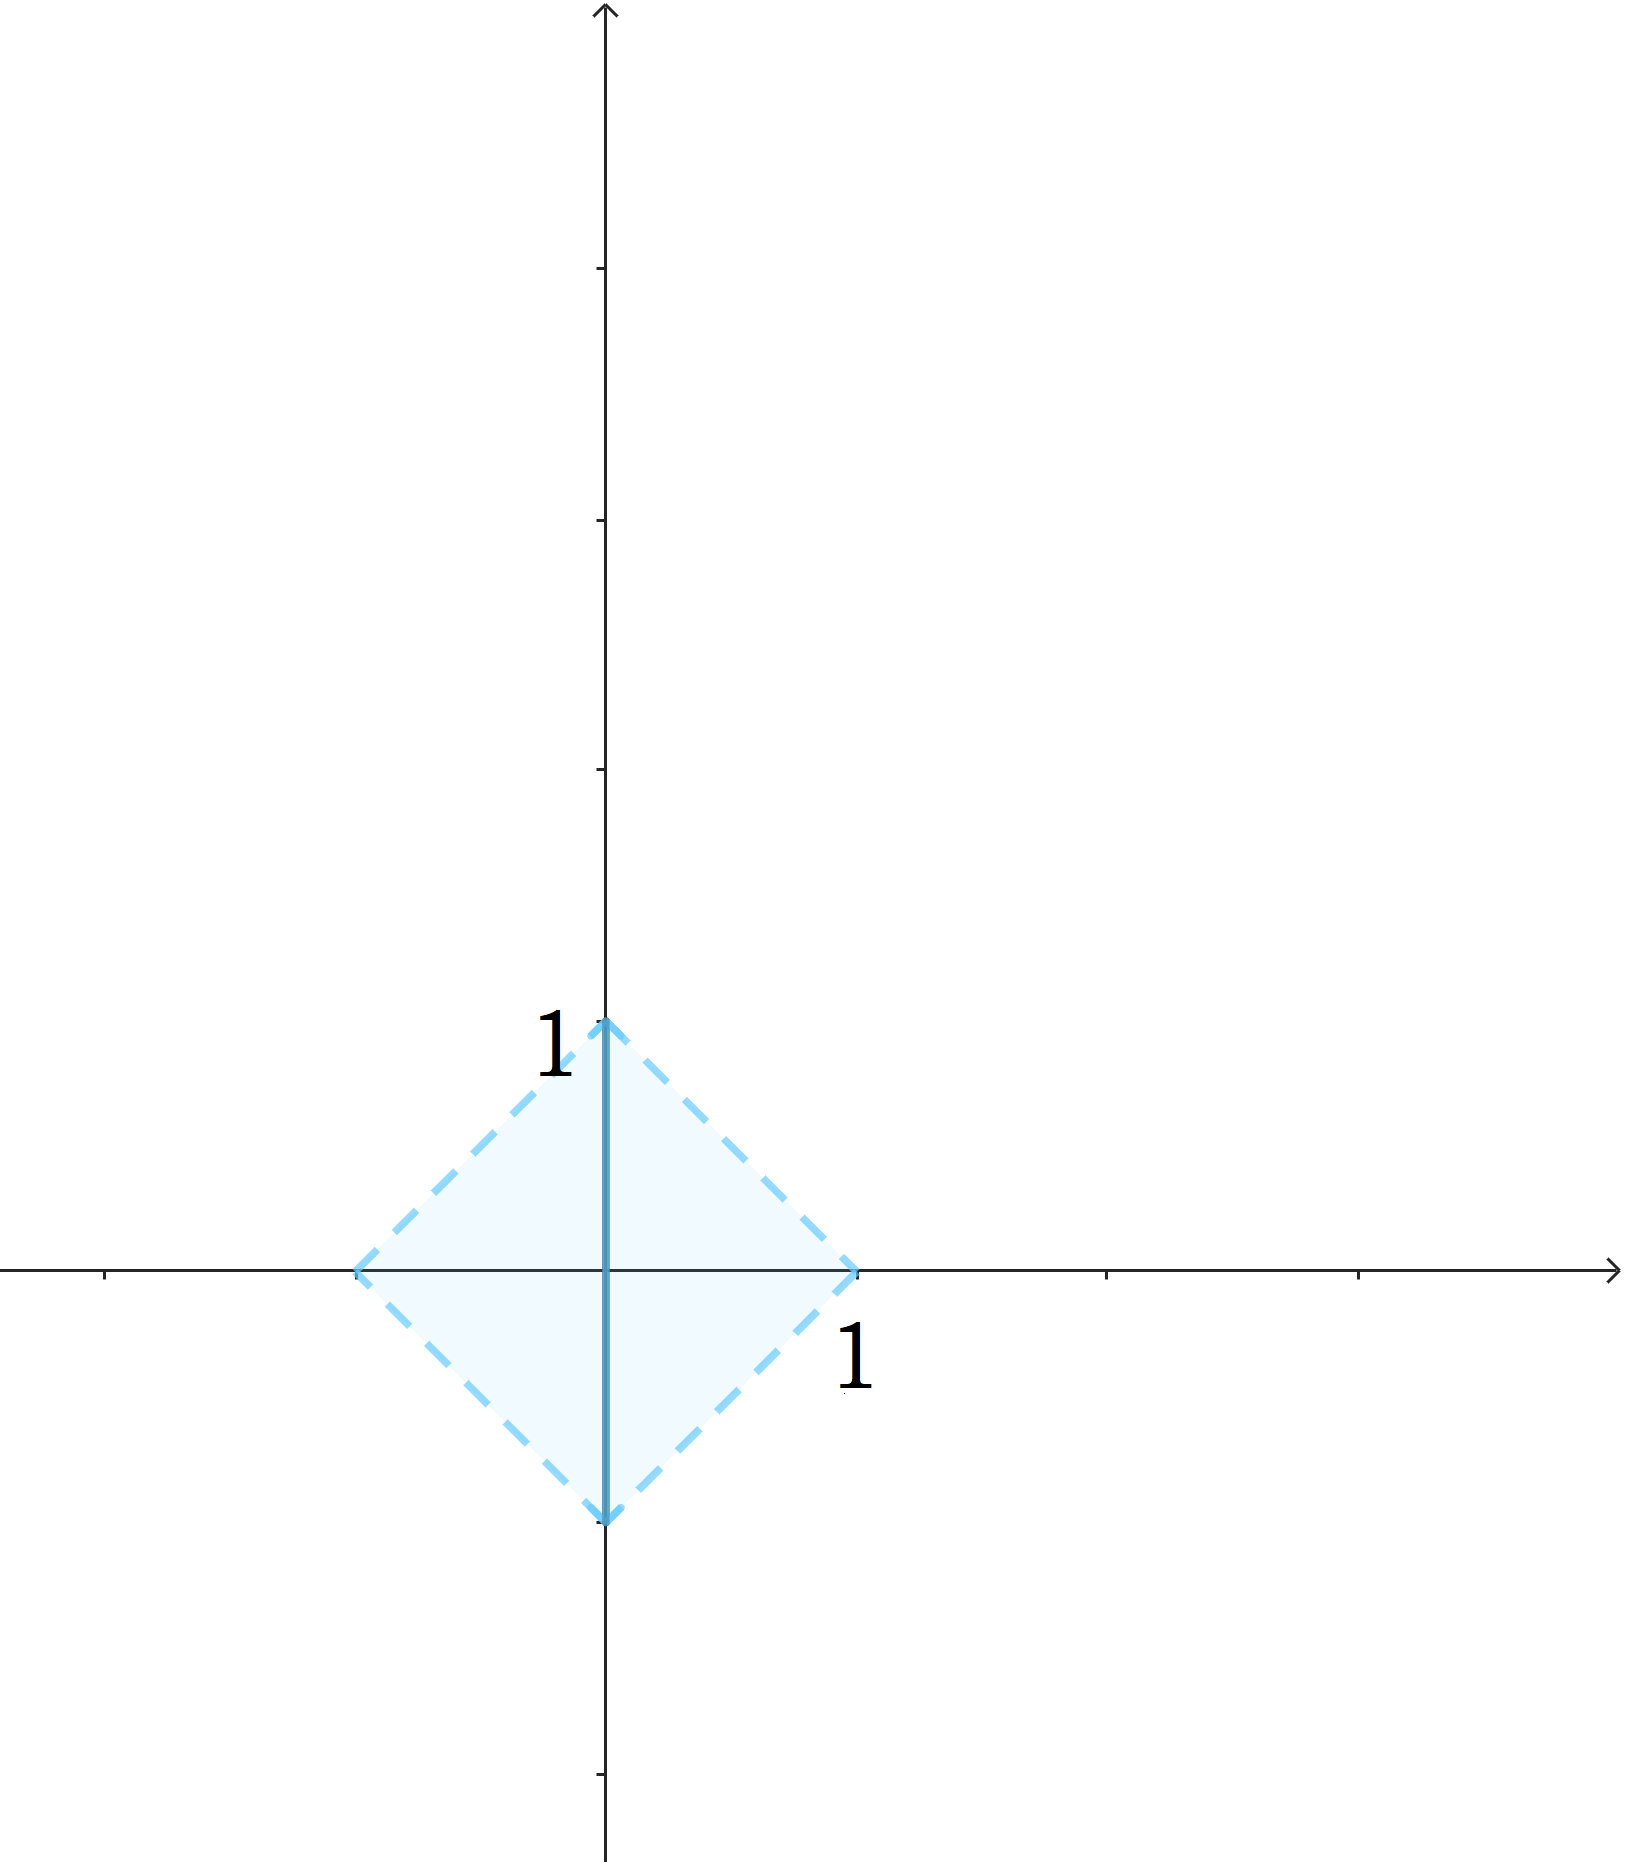
\includegraphics[scale=0.20] {graph7}
		\caption{\label{fig:7} Open ball $B((0,0), 1) $ in $\gamma$ metric }
	\end{figure}
	
	
	\begin{figure}
		\centering
		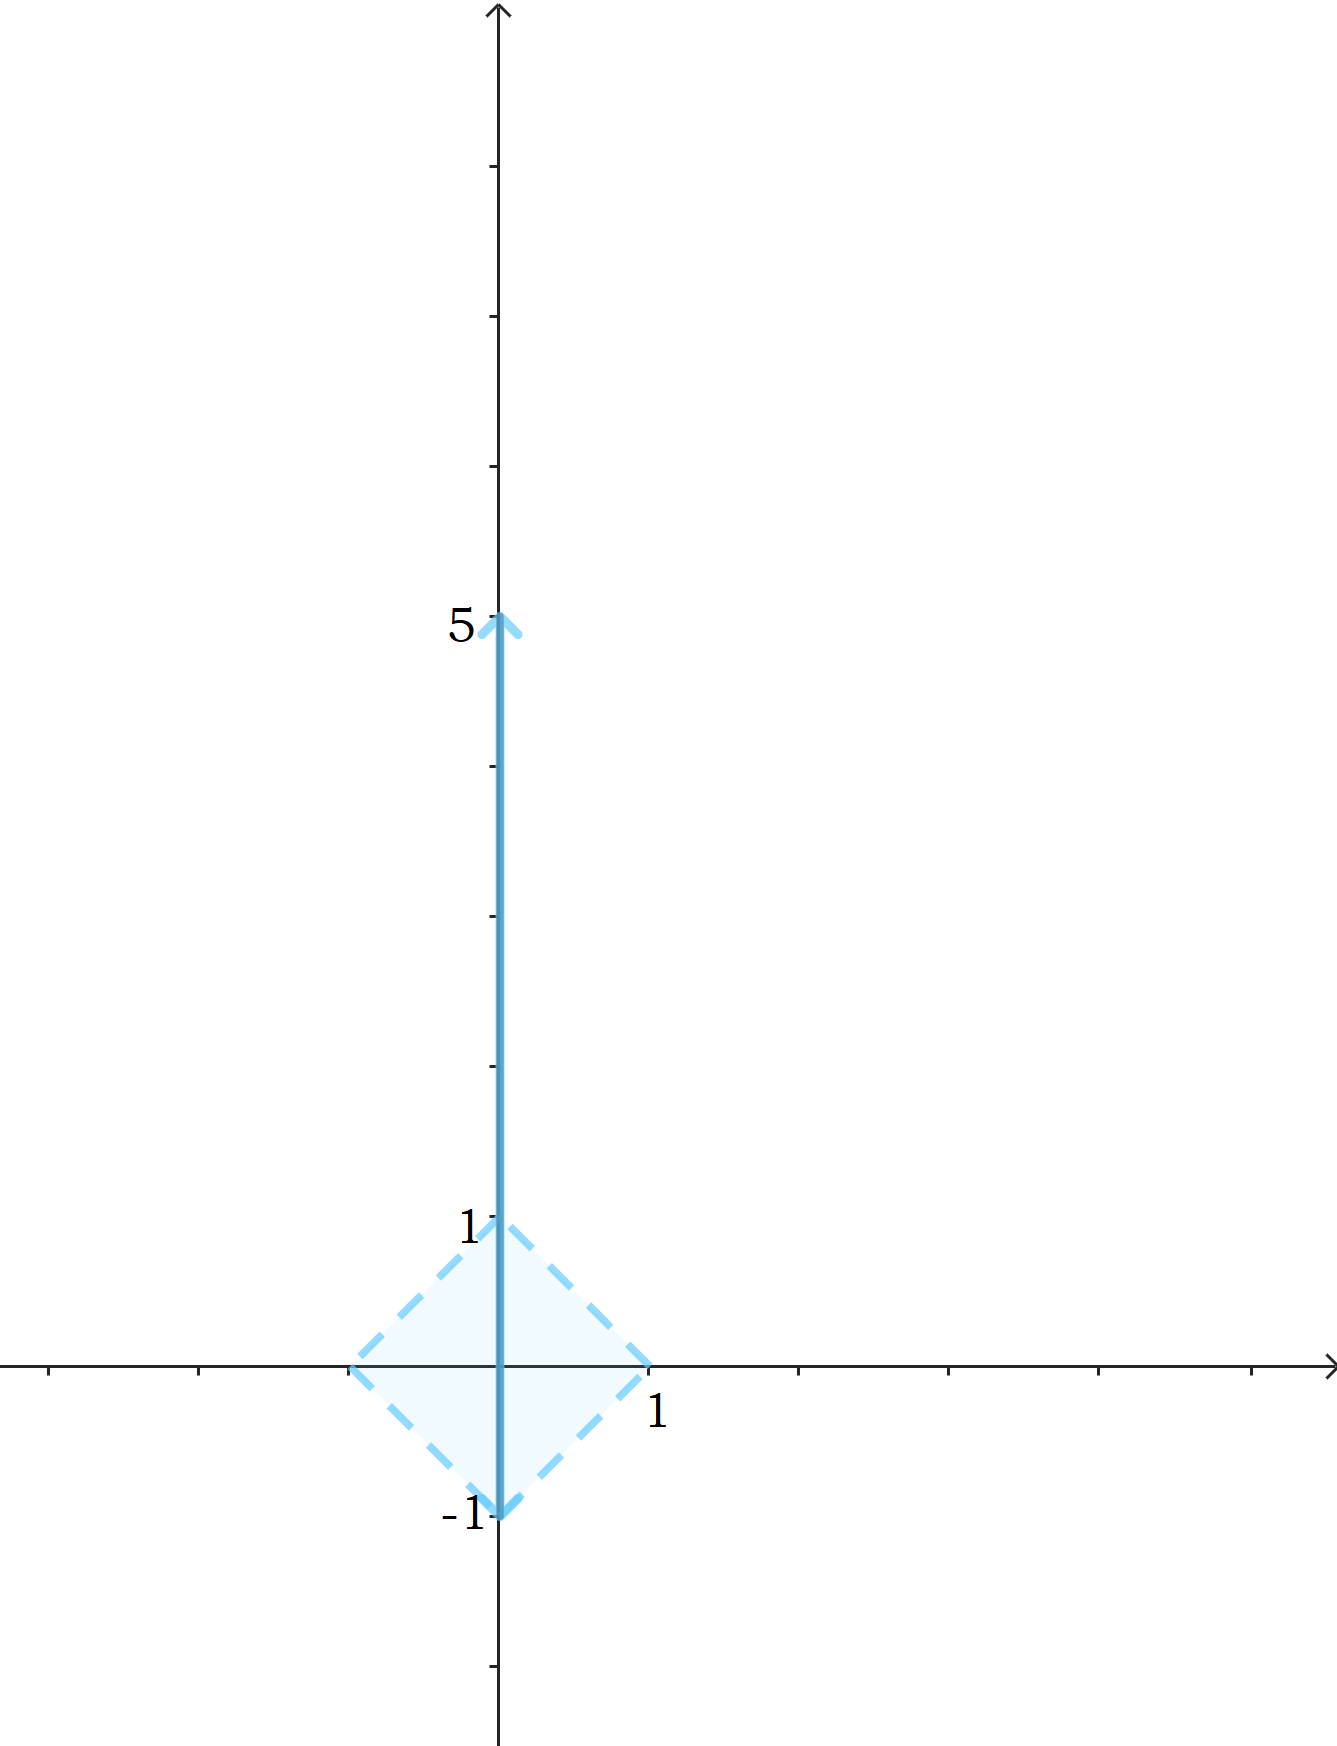
\includegraphics[scale=0.20] {graph8}
		\caption{\label{fig:8} Open ball $B((0,2), 3) $ in $\gamma$ metric }
	\end{figure}
	
	\begin{figure}
		\centering
		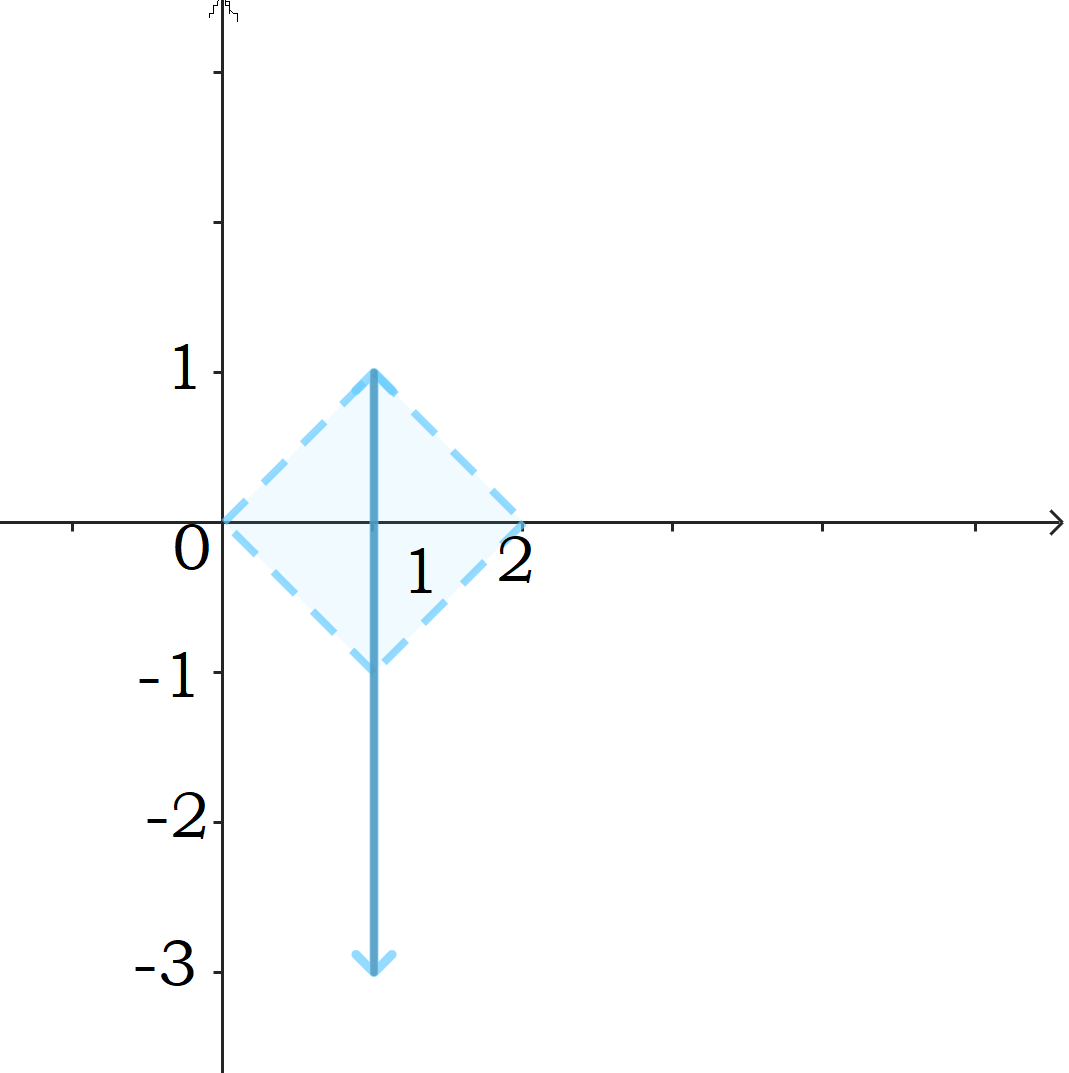
\includegraphics[scale=0.20] {graph9}
		\caption{\label{fig:9} Open ball $B((1,-1), 2) $ in $\gamma$ metric }
	\end{figure}
	\begin{align*}
		B((0,0), 1) &= \{(x_{1}, x_{2}) \in \mathbb{R}; \ \gamma((0,0),(x_{1}, x_{2}))<1\} \\
		&= \{(x_{1}, x_{2}) \in \mathbb{R}; \ x_{1} = 0 \land |x_{2}-0|<1\} \cup \{(x_{1}, x_{2}) \in \mathbb{R}; \ x_{1} \neq 0 \land |0| + |x_{1}-0| + |x{2}|<1\} \\
		&= \{(0, x_{2}) \in \mathbb{R}; \ \land \ |x_{2}|<1\} \cup \{(x_{1}, x_{2}) \in \mathbb{R}; \ x_{1} \neq 0 \land |x_{1}| + |x_{2}|<1\}
	\end{align*}

	\begin{align*}
	B((0,2), 3) &= \{(x_{1}, x_{2}) \in \mathbb{R}; \ \gamma((0,2),(x_{1}, x_{2}))<3\} \\
	&= \{(x_{1}, x_{2}) \in \mathbb{R}; \ x_{1} = 0 \land |x_{2}-2|<3\} \cup \{(x_{1}, x_{2}) \in \mathbb{R}; \ x_{1} \neq 0 \land |2| + |x_{1}-0| + |x{2}|<3\} \\
	&= \{(0, x_{2}) \in \mathbb{R}; \ \land \ |x_{2}-2|<3\} \cup \{(x_{1}, x_{2}) \in \mathbb{R}; \ x_{1} \neq 0 \land |x_{1}| + |x_{2}|<1\}
	\end{align*}

	\begin{align*}
		B((1,-1), 2) &= \{(x_{1}, x_{2}) \in \mathbb{R}; \ \gamma((1,-1),(x_{1}, x_{2}))<2\} \\
		&= \{(x_{1}, x_{2}) \in \mathbb{R}; \ x_{1} = 1 \land |x_{2}+1|<2\} \\
		&\cup \{(x_{1}, x_{2}) \in \mathbb{R}; \ x_{1} \neq 0 \land |-1| + |x_{1}-1| + |x{2}|<2\} \\
		&= \{(1, x_{2}) \in \mathbb{R}; \ \land \ |x_{2}+1|<2\} \cup \{(x_{1}, x_{2}) \in \mathbb{R}; \ x_{1} \neq 0 \land |x_{1}-1| + |x_{2}|<1\}
	\end{align*}
	

\subsection{Discrete metric} 
 \textbf{(a)}
    \begin{align*}
    	B(1,\frac{1}{2}) &= \{ x \in \mathbb{N}; d(1,x)<\frac{1}{2}\} \\
    	&= \{ x \in \mathbb{N}; x=1 \land 0<\frac{1}{2}\} \cup  \{ x \in \mathbb{N}; x \neq 1 \land d(1,x)<\frac{1}{2}\}  \\
    	&= \{1\} \cup \emptyset \\ 
    	&= \{1\}
    \end{align*}

 \begin{align*}
	B(2,1) &= \{ x \in \mathbb{N}; d(2,x)<1\} \\
	&= \{ x \in \mathbb{N}; x=2 \land 0<1\} \cup  \{ x \in \mathbb{N}; x \neq 2 \land d(2,x)<2\}  \\
	&= \{2\} \cup \emptyset \\ 
	&= \{2\}
\end{align*}

\begin{align*}
	\overline{B}(3,\frac{1}{2}) &= \{ x \in \mathbb{N}; d(3,x)\leq \frac{1}{2}\} \\
	&= \{ x \in \mathbb{N}; x=3 \land 0\leq \frac{1}{2}\} \cup  \{ x \in \mathbb{N}; x \neq 3 \land d(3,x)\leq \frac{1}{2}\}  \\
	&= \{3\} \cup \emptyset \\ 
	&= \{3\}
\end{align*}

\begin{align*}
	\overline{B}(4,1) &= \{ x \in \mathbb{N}; d(4,x)\leq 1\} \\
	&= \{ x \in \mathbb{N}; x=4 \land 0\leq1\} \cup  \{ x \in \mathbb{N}; x \neq 4 \land 1\leq 1\}  \\
	&= \{4\} \cup \mathbb{N} \setminus \{4\}\} \\ 
	&= \mathbb{N}
\end{align*}

In general, this discrete metric on space $X$ induces a metric space $(X,d)$ where the distance between any two pairwise distinct elements is $1$. Open and closed balls in this space contain one element or all of them:

\begin{equation*}
	B(x_{0}, r) =
	\begin{cases}
		\{x_{0}\} & 0 < r \leq 1\\
		 \mathbb{N} & r > 1\\
	\end{cases}       
\end{equation*}

\begin{equation*}
	\overline{B}(x_{0}, r) =
	\begin{cases}
		\{x_{0}\} & 0 < r < 1\\
		\mathbb{N} & r \geq 1\\
	\end{cases}       
\end{equation*}

\textbf{(b)} Because the distance between any two pairwise distinct elements is $1$, every triangle $abc$ with pairwise distinct elements $a$, $b$ and $c$ is equilateral (all three edges have the same lenght 1).

\subsection{Homeomorphic spaces} 
In this exercise I was working with spaces $X_{n} = S^{n-1} \times [0,1] \subset \mathbb{R}^{n+1}$ and $Y_{n}=\{(x_{1},  ... , x_{n}) \in \mathbb{R}^n; 1 \leq x_{1}^2 + ... + x_{n}^2 \leq 4 \}$. \\

\noindent Spaces $X_{1}$, $Y_{1}$, $X_{2}$, $Y_{2}$ that I've drawn can be seen on Figures 10, 11, 12 and 13. \\

\begin{figure}
	\centering
	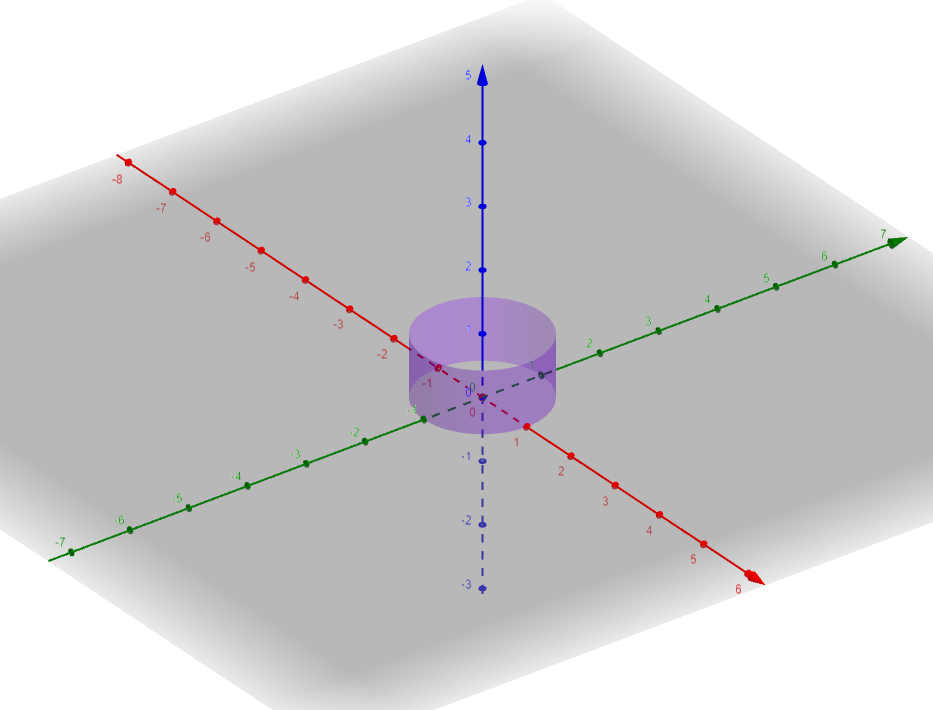
\includegraphics[scale=0.40] {graph10}
	\caption{\label{fig:10} $X_{2}$ space}
\end{figure}


\begin{figure}
	\centering
	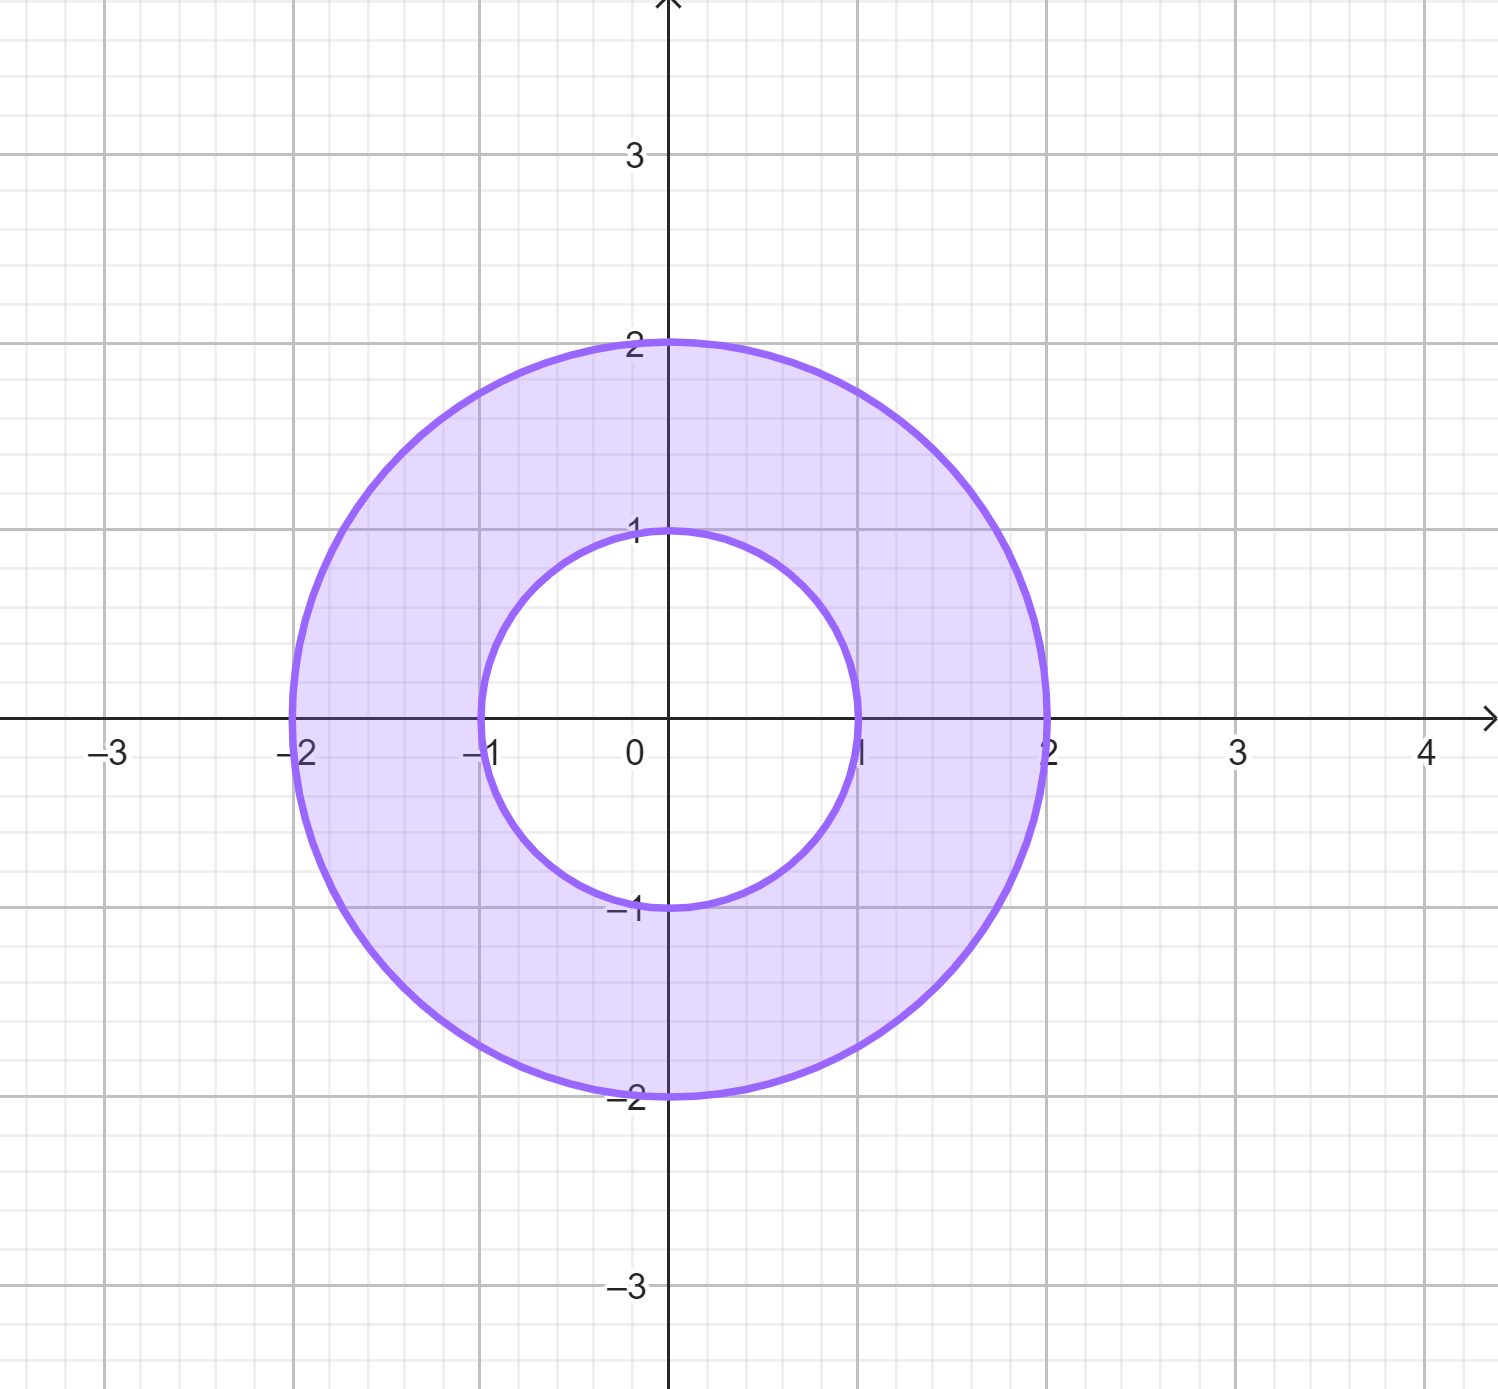
\includegraphics[scale=0.20] {graph11}
	\caption{\label{fig:11} $Y_{2}$ space}
\end{figure}

\begin{figure}
	\centering
	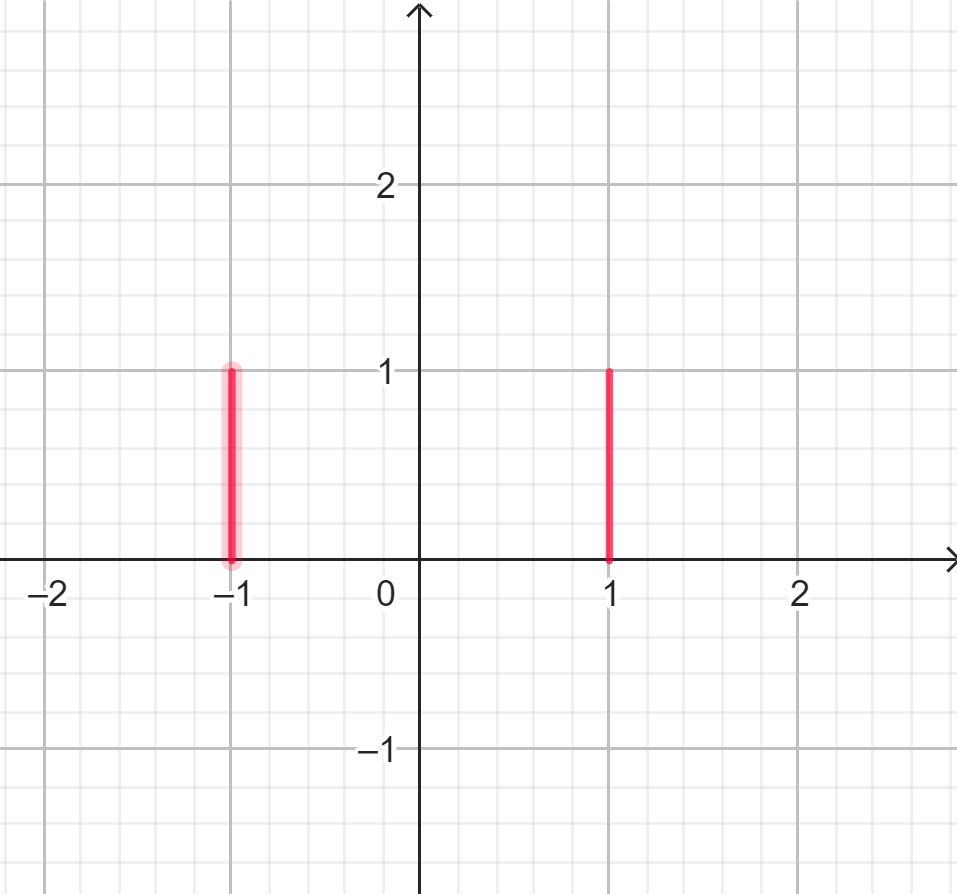
\includegraphics[scale=0.20] {graph12}
	\caption{\label{fig:12} $X_{1}$ space }
\end{figure}

\begin{figure}
	\centering
	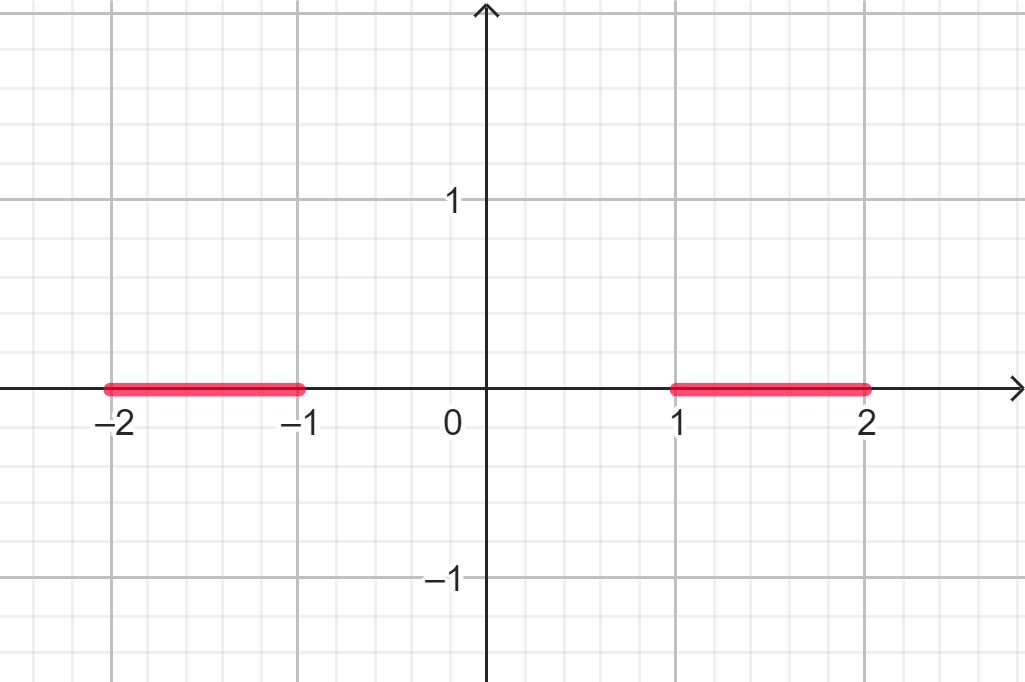
\includegraphics[scale=0.20] {graph13}
	\caption{\label{fig:13} $Y_{1}$ space }
\end{figure}

\noindent I got the inspiration for the proof for a general $n$ from the solved problems book by asist. dr. Aleksandra Franc (2) on spletna učilnica where lies the proof for $n=2$. I generalized the idea for $n \in \mathbb{N}$. \\


\noindent In my proof I used the following theorem from the lectures: \\

\noindent \textbf{Theorem} Let $X$ and $Y$ be topological spaces. If we can find continuous maps $f : X \rightarrow Y$ and $g : Y \rightarrow X$ such that $f \circ g = id_{Y}$ and $g \circ f = id_{X}$, then X and Y are homeomorphic. \\

\noindent \textbf{Proof that $X_{n}$ and $Y_{n}$ are homeomorphic for any $n \in \mathbb{N}$:} \\

\noindent First I rewrote $X_{n}$ as: \\
$$X_{n}=\{(x_{1},  ... , x_{n+1}) \in \mathbb{R}^{n+1}; \  x_{1}^2 + ... + x_{n}^2 = 1, \ 0 \leq x_{n+1} \leq 1 \}$$ \\
\noindent Next, I defined two functions $f$ and $g$ and then used the beforementioned theorem.   \\

\noindent I defined $f: X_{n} \rightarrow Y_{n}$ as:  \\
$$f(x_{1},...,x_{n+1}) = ((x_{n+1} + 1) \cdot x_1, ... , (x_{n+1} + 1) \cdot x_1, (x_{n} + 1) \cdot x_{n+1} )$$


\noindent The idea was that I took the last coordinate, added 1 and multiplied it with other coordinates to lower the dimension. It is the same idea as for $n=2$, where we mapped surface to the plane. The proof that $f$ is well defined ($f(x_{1},...,x_{n+1}) \in Y_{n}$): \\

\noindent Let $(x_{1},...,x_{n+1}) \in X_{n}$. That means $x_{1}^2 + ... + x_{n}^2 = 1$ and $0 \leq x_{n+1} \leq 1$. Subsequently: 

	\begin{align*}
((x_{n+1} + 1) \cdot x_{1})^2 + ... +  ((x_{n+1} + 1) \cdot x_{n})^2
&= (x_{n+1} + 1)^2 \cdot x_{1}^2 + ... +  (x_{n+1} + 1)^2 \cdot x_{n}^2  \\
&= (x_{n+1} + 1)^2 \cdot (x_1^2 + ... + x_n^2) \\
&=  (x_{n+1} + 1)^2 \cdot 1 \\
&=  (x_{n+1} + 1)^2 
\end{align*}

\noindent Because $0 \leq x_{n+1} \leq 1$ it holds that: 

$$1 \leq (x_{n+1} + 1)^2  \leq 4$$

\noindent And so: $f(x_{1},...,x_{n+1}) \in Y_{n}$ \\



\noindent I also defined $g: Y_{n} \rightarrow X_{n}$ as:  \\
$$g(x_{1},...,x_{n}) = (\frac{x_1}{\sqrt{x_1^2 + ... + x_n^2}}, ... ,  \frac{x_n}{\sqrt{x_1^2 + ... + x_n^2}}, \sqrt{x_1^2 + ... + x_n^2} - 1)$$

\noindent The idea was to make every vector from origin to point unit by dividing it with Euclidean distance $||x_{1},...,x_{n}||_2 = \sqrt{x_1^2 + ... + x_n^2}$ from origin to its ending point and instead express their lenght in the last coordinate. I wrote $r =||x_{1},...,x_{n}||_2$. The proof that $g$ is well defined $g(x_{1},...,x_{n}) \in X_{n}$: \\

\noindent Let $(x_{1},...,x_{n}) \in Y_{n}$. 

\begin{align*} 
	\left(\frac{x_1}{\sqrt{x_1^2 + ... + x_n^2}}\right) ^2 \ + \ ... \ + \ \left(\frac{x_n}{\sqrt{x_1^2 + ... + x_n^2}}\right)^2
	&= \frac{x_1^2}{r^2} + ... + \frac{x_n^2}{r^2} \\
	&= \frac{x_1^2 + ... + x_n^2}{r^2}	\\
	&= \frac{x_1^2 + ... + x_n^2}{x_1^2 + ... + x_n^2} \\
	&= 1
\end{align*}

\noindent Because $1 \leq x_{1}^2 + ... + x_{n}^2 \leq 4$ it holds that: 


\begin{align*} 
1 &\leq \sqrt{x_1^2 + ... + x_n^2} &\leq 2 \\
0 &\leq \sqrt{x_1^2 + ... + x_n^2} - 1 &\leq 1
\end{align*}

\noindent And so $g$ is well defined. \\

\noindent The proof that $f \circ g = id_{Y_n}$:
\begin{align*}
	f(g(x_1,...,x_n)) &= f(\frac{x_1}{r}, ... , \frac{x_n}{r}, r-1) \\
	&= ((r-1+1) \cdot \frac{x_1}{r},...,(r-1+1) \cdot \frac{x_n}{r}) \\
	&= (r \cdot \frac{x_1}{r},..., r \cdot \frac{x_n}{r}) \\
	&= (x_1,..., x_n)
	\end{align*}

\noindent The proof that $g \circ f = id_{X_n}$:

\noindent In my computation are used the following preconditions: $x_{1}^2 + ... + x_{n}^2 = 1, \ 0 \leq x_{n+1} \leq 1$.

\begin{align*}
	\sqrt{(x_{n+1} + 1)^2 \cdot x_1 ^2+...+(x_{n+1}+1)^2 \cdot x_n^2}  & = \sqrt{(x_{n+1}+1)^2(x_1^2 + ... + x_n^2)} \\
	&= \sqrt{(x_{n+1}+1)^2 \cdot (x_1^2 + ... + x_n^2)} \\
	&= \sqrt{(x_{n+1}+1)^2 } \\
	&= |(x_{n+1}+1)| \\
	&= (x_{n+1}+1)
\end{align*}


\begin{align*}
	g \circ f &= g(f(x_1,...,x_n,x_{n+1})) \\
	&= g((x_{n+1}+1)x_1,...,(x_{n+1}+1)x_n) \\
	&= \left( \frac{(x_{n+1}+1)x_1}{x_{n+1}+1},...,\frac{(x_{n+1}+1)x_n}{x_{n+1}+1}, x_{n+1}+1-1 \right) \\
	&= (x_1, ...,x_n,x_{n+1})
\end{align*}

\qed

	\section{Programming problems}
\subsection{ Deciding connectivity} 
To find connected components in graph I used the dfs algorithm. My program graphcomponents.py consists of function findComponents. Its inputs are list of vertices V and list of edges E. Inside function there is another function, named dfs, which is defined only locally. Its inputs are vertex, graph that is a set of edges and set named visited, that contains vertices already visited by the dfs algorithm. Dfs algorithm searches through the vertices and edges and add visited vertices in visited set. Visited vertices are part of one of the connected components. In the main while loop function dfs is called on every iteration and list of components is updated with lists of visited vertices until there are no more vertices left in the graph. Vertices in components are sorted by numbers from the smallest to the greatest.

\noindent I tested my program on five different test cases (one of them can be seen on Figure 14):  \\

\begin{figure}
	\centering
	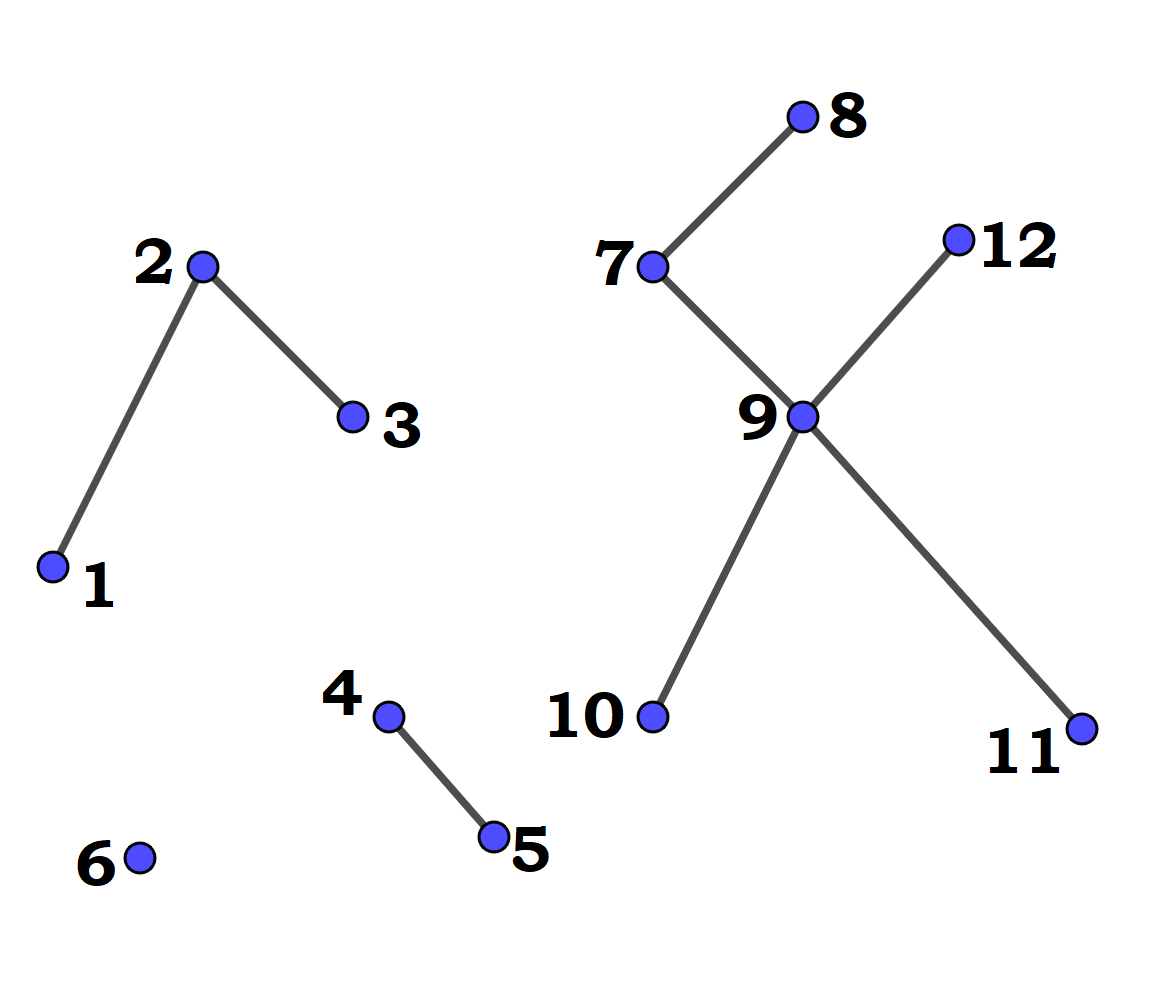
\includegraphics[scale=0.30] {graph14}
	\caption{\label{fig:14} Testing case in Deciding connectivity problem.}
\end{figure}

\noindent $V = [1, 2, 3, 4, 5, 6, 7, 8] $ \\
$E = [(1, 2), (2, 3), (1, 3), (4, 5), (5, 6), (5, 7), (6, 7), (7, 8)]$ \\
$findComponents(V, E) = [[1, 2, 3], [4, 5, 6, 7, 8]] $ \\

\noindent $V = [1, 2, 3, 4, 5]$ \\
$E = [(1, 2), (1, 3), (1, 4), (1, 5)]$ \\
$findComponents(V, E) = [[1, 2, 3, 4, 5]] $ \\

\noindent $V = [1, 2, 3, 4, 5, 6, 7, 8, 9] $ \\
$E = [(1, 2), (1, 3), (1, 8), (3, 7), (4, 5), (4, 6), (4, 9), (5, 6), (5, 9), (7, 8)]$ \\
$findComponents(V, E) = [[1, 2, 3, 7, 8], [4, 5, 6, 9]] $ \\

\noindent $V = [1, 2, 3, 4, 5] $ \\
$E = []$ \\
$findComponents(V, E) = [[1], [2], [3], [4], [5]] $ \\

\noindent $V = [1, 2, 3, 4, 5, 6, 7, 8, 9, 10, 11, 12] $ \\
$E = [(1, 2), (2, 3), (4, 5), (7, 8), (7, 9), (9, 10), (9, 11), (9, 12)]$ \\
$findComponents(V, E) = [[1, 2, 3], [4, 5], [6], [7, 8, 9, 10, 11, 12]] $ \\

\subsection{Shelling discs} 

My file shelling.py contains function shelling(T) that outputs 










 
    
    
    
    
    
	
	\bibliographystyle{unsrt}
	\bibliography{references}
	
	
	
	% --------------------------------------------------------------
	%     You don't have to mess with anything below this line.
	% --------------------------------------------------------------
	
	
\end{document}    
